\documentclass[10pt]{article}
\usepackage{fullpage}
\usepackage{epsf}
\usepackage{amsmath}
\usepackage{amsthm}
\usepackage{txfonts,pxfonts,amsfonts}
\usepackage{epsfig}
\usepackage{caption}
% \usepackage{subfig}
\usepackage{graphicx}
\usepackage[citecolor=blue,linkcolor=blue,colorlinks=true]{hyperref}
% \usepackage{algorithmic}
% \usepackage{algorithm}

\usepackage{booktabs} % For formal tables
\usepackage{xspace}
\usepackage{lipsum}
\usepackage{courier}
\usepackage{array,multirow}
\usepackage{float}
\usepackage{wrapfig}

\usepackage{subcaption}
% \usepackage{hyperref}
\usepackage{listings}
\usepackage[ruled,linesnumbered]{algorithm2e}
\usepackage{url}

\usepackage{tikz}
\usetikzlibrary{arrows,shapes.geometric,positioning,shapes.multipart,matrix,calc,patterns}
    \usetikzlibrary{topaths}
\usetikzlibrary{decorations.text}
\usepackage{pgfplots}
\usepackage{color}
\usepackage{pgfplotstable}


\lstset{
  escapeinside={\`}{\`}
}
\lstdefinestyle{rm}{mathescape,basicstyle=\normal\ttfamily}


\newcommand{\hlight}[1]{{\em #1}}
\newcommand{\REM}[1]{}
\newcommand{\name}{{\tt Falcon-Bi}\xspace}
\newcommand{\Graph}{\texttt{Graph}\xspace}
\newcommand{\GPU}{\texttt{GPU}\xspace}
\newcommand{\CPU}{\texttt{CPU}\xspace}
\newcommand{\Point}{\texttt{Point}\xspace}
\newcommand\UK[1]{\textcolor{red}{#1}}
\newcommand{\Edge}{\texttt{Edge}\xspace}
\newcommand{\todo}[1]{\color{blue}{#1}}


\def\reporttitle{Custom Code Generation for a Graph DSL}
\def\reportauthor{Bikash Gogoi}
\def\authorrollno{CS14B039}
\def\guide{Dr.~Rupesh Nasre (Dept of Computer Science \& Engineering, IIT Madras)}


\title{\reporttitle \\ {\small (Dual Degree Project - Interim Report)}}
\author{\reportauthor\ (\authorrollno)~\footnote{Guide : \guide}}
\date{\today}

\begin{document}
\maketitle

\begin{abstract}
We present challenges faced in making a domain-specific language (DSL) for graph algorithms adapt to varying requirements to generate a spectrum of efficient parallel codes. Graph algorithms are at the heart of several applications, and achieving high performance with them has become critical due to tremendous growth of irregular data. However, irregular algorithms are quite challenging to parallelize automatically, due to access patterns influenced by the input graph -- which is unavailable until execution. Former research has addressed this issue by designing DSLs for graph algorithms, which restrict generality, but allow efficient code-generation for various backends. Such DSLs are, however, too rigid, and do not adapt to changes in backends or to input graph properties or to both. We narrate our experiences in making an existing DSL, named Falcon, adaptive. The biggest challenge in the process is to not change the DSL code for specifying the algorithm. We illustrate the effectiveness of our proposal by auto-generating codes for vertex-based versus edge-based graph processing, synchronous versus asynchronous execution, and CPU versus GPU backends.
\end{abstract}

\newpage
\tableofcontents
\newpage
\section{Introduction}\label{sec:introduction}
\subsection{Motivation}
Graphs model several real-world phenomena such as friendship, molecular interaction and co-authorship.
Several graph algorithms have been designed across domains to compute such relationships between entities.
Performance of these graph algorithms has become critical today due to explosive growth of unstructured data.
For instance, to simulate a simple physical phenomenon, an algorithm may have to work with billions of particles.

On the other side, computer hardware is witnessing rapid changes with new architectural innovations.
Exploiting these architectures demands complex coding and good compiler support.
The demand intensifies in the presence of parallelization.
It is not uncommon to see a twenty-line textbook graph algorithm implemented using several hundred lines of optimized parallel code.

It would be ideal if the algorithm is programmed at a high-level without worrying about the nuances of the hardware.
This gave rise to domain-specific languages (DSLs) for graph algorithms which allowed programmers to write complex algorithmic codes and took care of efficient parallel code generation~\cite{greenmarl, lighthouse, falcon}.
Such DSLs often disallow writing arbitrary programs, trading off generality for performance.
This makes programming parallel hardware easy, and adapting to changes manageable.

An example of a graph DSL is Falcon~\cite{falcon, dhfalcon} which supports a wide variety of backends: CPU, GPU, multi-GPU, heterogeneous processing, and distributed systems. 
It extends C language to allow graph processing being specified at a high-level.
Falcon provides special constructs (such as worklists and reductions) for simplifying algorithm specification and also aiding efficient code generation.
We choose Falcon because it supports a variety of backends.

Unfortunately, graph algorithms do not always have a fixed performance pattern.
The pattern varies depending upon the graph structure which is available only at runtime.
Such an \textit{irregular} pattern poses challenges in parallelizing graph algorithms and in optimizing them for efficient execution.
For instance, vertex-based processing works well for road networks, but social networks demand an edge-based processing.
Sequential processing of parallel loops demands synchronous execution, but independent loops can be more efficient with asynchronous processing.
Similarly, backend optimizations are quite different for different targets such as CPU and GPU.

Falcon (and other graph DSLs) allows writing code for a particular kind of processing. % UK- this is true for other DSLs, so ours is novel as such a dsl is lacking. needs to be highlighted.
The code written in Falcon DSL needs modifications for an alternative way of processing.
Various syntactic elements in the program need to be changed for the alternative way. 
Thus, code needs to be written separately for vertex-based and edge-based processing, for instance.
While this is a step better than being totally rigid, it would be helpful if one could generate different kind of code from the \textit{same DSL specification}.
Such a setup greatly simplifies algorithmic specification, and also allows generating code for various situations / backends / graph types from the same specification.

The burden, in this setup, shifts from DSL programmer to the compiler.
The only input that the programmer needs to specify (apart from the DSL code) is the type of processing required.
This can be easily specified via a command-line switch (e.g., \texttt{-vertex-based}, -\texttt{synchronous}, etc.), but without needing any modifications to the code.
This allows our compiler to generate vertex-based and edge-based graph processing code from the same algorithmic specification.
Similarly, it allows generating synchronous and asynchronous processing code, wherein various iterations of the parallel processing are separated and not separated by a barrier respectively. % UK - synchronous and asynchronous needs expansion here. our targeted platform - multi-gpu machine needs to be mentioned.
The compiler is also equipped to generate CPU or GPU or multi-GPU code.

\subsection{Our Contribution}
In this report, we highlight the challenges faced in keeping the specification fixed.
In particular, we make the following contributions:
\begin{itemize}
\item We present a compiler which generates different implementations for the \textit{same DSL program} for an algorithm which differ in graph processing. In particular, the compiler can generate vertex-based or edge-based processing, synchronous or asynchronous codes, and CPU or GPU or multi-GPU codes.
\item The DSL is able to manage multiple GPUs present in a multi-GPU machine by adding support for running programs in parallel which differ in algorithm or input graph.
\item We illustrate the effectiveness of the proposed compiler using several graph algorithms and several graphs of various types. The performance of the code generated with the proposed compiler is compared against other hand-tuned as well as generated codes.
\end{itemize}

\subsection{Outline}
The rest of the report is organized as below.
Chapter~\ref{sec:background} provides a brief background of Falcon DSL, as our work adds facilities in it.
Chapter~\ref{sec:approach} presents challenges faced in generating various codes from the same DSL.
Chapter~\ref{sec:results} evaluates the effectiveness of our approach using multiple frameworks, algorithms and graphs.
Chapter~\ref{sec:related} compares and contrasts the relevant related work,
and Chapter~\ref{sec:conclusion} concludes.

\newpage
\section{Background}\label{sec:background}
We provide a comparison of a few graph frameworks, followed by a brief background on Falcon.

\subsection{Comparison of Different Graph Frameworks}
Table~\ref{background:table1} differentiates various graph data analytic tools based on programming style, hardware support and processing style. 

%GPUs and Multi-GPU machines are not rare now and GPGPU has attracted every field of computation.
%\newline\UK{UK- words  coalesced access, SIMT, MIMD, thread divergence etc., should come here?}\newline
 Galois~\cite{Pingali:2011:TPA:1993316.1993501} is a framework for graph algorithms.
\REM{ works only for multi-core CPUs.} 
It iterates over a collection  of active elements which are stored in a worklist.
After one parallel iteration over a worklist, new active elements are generated which are stored in another worklist for next iteration.
Program terminates when no new active elements are generated during an iteration.
Galois supports different types of worklists. It supports dynamic algorithms, where graph structure changes at runtime.
Green-Marl~\cite{Hong:2012:GDE:2150976.2151013} is a Graph DSL. 
\REM{Green-Marl DSL allows programming only for multi-core CPUs.}
The DSL supports various  data types,  parallel constructs to  iterate over graph, synchronization and reduction functions. 
This makes programming  graph algorithms using Green-Marl DSL easy.  
Galois and Green-Marl target multi-core CPUs and do not support \GPU devices.

LonestarGPU~\cite{nasre13:MAG:2517327.2442531} framework supports  dynamic algorithms. %\UK{need to define cautious, even in Galois?} 
It has  implementations of dynamic graph algorithms such as Delaunay
Mesh Refinement and Survey Propagation. Static graph algorithms such as SSSP, BFS, Connected Components etc., are also programmed in LonestarGPU.
Being a framework (and not a DSL), programming new algorithm in LonestarGPU require expertise in CUDA and  framework code. 
Gunrock~\cite{Wang:2016:GHG:3016078.2851145} has a set of APIs to express a
wide range of graph processing primitives on GPUs. %It also has some GPU-specific optimizations.
It defines {\it frontiers} as a subset of edges and vertices of the graph which are actively involved
in the computation. Gunrock defines \textsf{advance}, \textsf{filter}, and \textsf{compute} primitives which operate on
frontiers in different ways. 
Similar to LonestarGPU, Gunrock is a library-based framework and, relative to DSLs, programming is difficult. 

Falcon~\cite{falcon} is a Graph DSL which supports \CPU, \GPU and multi-GPU machines. It supports various data types, parallelization and synchronization constructs, and reduction operations. This makes programming graph analytic algorithms easy for heterogeneous targets. Falcon also supports dynamic graph algorithms. 
Totem~\cite{Gharaibeh:2012:YOT:2370816.2370866} is  a library-based framework consisting of benchmarks which can run on \CPU, \GPU and multi-GPU machines. Programming new algorithms in Totem is relatively tougher.

\begin{table}
\centering
\scalebox{0.7}{
 \begin{tabular}{|p{2.0cm}|p{1cm}| p{3.5cm}| p{3.5cm}|}
\hline
\small
Tool & DSL & \shortstack {Hardware Support\\ \CPU : \GPU : multi-GPU} & \shortstack{ Iterators \\ Edge : Vertex : Worklist} \\
\hline
\hline
GreenMarl & $\surd$ & $\surd$\hspace{0.08in} : $\times$\hspace{0.1in} : $\times$ & $\surd$\hspace{0.08in} : $\surd$\hspace{0.1in} : $\surd$\\
%\hline
Galois & $\times$ & $\surd$\hspace{0.08in} : $\times$\hspace{0.1in} : $\times$ & $\times$\hspace{0.08in} : $\times$\hspace{0.1in} : $\surd$\\
%\hline
Falcon & $\surd$ & $\surd$\hspace{0.08in} : $\surd$\hspace{0.1in} : $\surd$ & $\surd$\hspace{0.08in} : $\surd$\hspace{0.1in} : $\surd$\\
%\hline
Totem & $\times$ & $\surd$\hspace{0.08in} : $\surd$\hspace{0.1in} : $\surd$ & $\times$\hspace{0.08in} : $\times$\hspace{0.1in} : $\times$\\
%\hline
Gunrock & $\times$ & $\times$\hspace{0.08in} : $\surd$\hspace{0.1in} : $\times$ & $\times$\hspace{0.08in} : $\times$\hspace{0.1in} : $\surd$\\
%\hline
LonestarGPU & $\times$ & $\times$\hspace{0.08in} : $\surd$\hspace{0.1in} : $\times$ & $\surd$\hspace{0.08in} : $\surd$\hspace{0.1in} : $\surd$\\
\hline
\end{tabular}
}
\caption{Comparison of different graph frameworks}
\label{background:table1}
\end{table}

As shown in  Table~\ref{background:table1}, both Green-Marl and Falcon support iteration over nodes and edges. Falcon supports multiple hardware platforms. So we have taken Falcon DSL for implementing our compilation strategies where several optimizations are performed. These optimizations are missing in any of the current graph DSL. By retaining the DSL code intact for various transformations, our compiler considerably reduces the programming effort and improves productivity.

\subsection{Falcon}
Falcon Graph DSL has data types {\tt Graph}, {\tt Point}, {\tt Edge}, {\tt Set} and {\tt Collection}. \texttt{Graph} stores a graph object, which consist of points and edges. Each {\tt Point} is stored as {\tt union} of   {\tt int} and {\tt float}.
{\tt Edge} consist of source and destination points and  a {\it weight}. {\tt Set} is a static collection and implemented as a {\it Union-Find} data structure. The {\tt Collection} data type is dynamic and its size can vary at runtime. Elements can be added to  and deleted from a collection object at runtime.

 The {\tt foreach} statement is the parallelization construct of Falcon.
 It can be used to  iterate in different ways on different elements of graph object as  shown in Table~\ref{background:tabfalcon2}. 
{\tt Parallel} {\tt  Sections} statement of Falcon is used to write programs which uses multiple devices of a machine at the same time. Falcon also supports reduction operations such as add ({\it RADD}) and mul ({\it RMUL}). It  has atomic library functions {\it MIN}, {\it MAX} etc., which are necessary for graph algorithms as they are {\it irregular}. 
The synchronization primitive of Falcon DSL is {\tt single} statement.
 It is a non-blocking lock and can be used to lock one element or a collection of elements, as shown in Table~\ref{background:tabfalcon1}.

\begin{table}
%\small
 \small{
\centering
\begin{tabular}{ |l |l |l| }
 \hline
  Data Type &Iterator  & Description  \\
\hline
  Graph   &  points  &  Iterate over  all points in graph \\
%\hline
Graph    & edges    & Iterate over all edges in graph \\
% \hline
%Graph   & pptyname  & Iterate over all elements in new ppty (e.g triangles in a  mesh).\\
%\hline
Point   & nbrs     & Iterate over all neighboring points (Undirected {\tt Graph})\\
%\hline
Point   & innbrs     & Iterate over all src point of incoming edges\\
%\hline
Point   & outnbrs   & Iterate over dst   point of   outgoing  edges \\
%\hline
Set     &      & Iterate over all items in a Set \\
%\hline
Collection       &    & Iterate over all items in a Collection\\
\hline
\end{tabular}
\caption{ {\tt foreach}  statement iterators in Falcon}
\label{background:tabfalcon2}
}
\vspace{2em}
\small{
\centering

 \begin{tabular}{|l|l|}
 %\begin{tabular}{|p{2cm}|p{5cm}|}
\hline
\shortstack{ \textbf{single}(t1) \{stmt block1\}\\ \textbf{else} \{stmt block2\}}  &\shortstack{ The thread that gets a lock on  item t1\\ executes  stmt block1 and other threads\\ execute stmt block2.}\\
\hline
\shortstack{ \textbf{single}(coll) \{stmt block1\}\\ \textbf{else} \{stmt block2\}}  & \shortstack{The thread that gets a lock on  all elements\\ in the collection executes  stmt block1\\ and others execute stmt block2.}\\
\hline
 \end{tabular}
\caption{{\tt single} statement (synchronization) in Falcon}
\label{background:tabfalcon1}
}

\end{table}


A graph object can be processed in multiple ways in Falcon. This leads to the flexibility of the same algorithm being specified in different ways.   A programmer can iterate over {\it edges} of a graph object and then extract the source ({\it src}) and the destination ({\it dst}) points of each edge. Another method is to iterate over all {\it points} of the graph object. 
Then for each point, the processing can iterate over {\it outnbrs} or {\it innbrs}.
This is illustrated in Algorithms~\ref{background:algo1} and \ref{background:algo2}.

% \begin{wrapfigure}{L}{0.6\textwidth}
\begin{figure}
\begin{minipage}[t]{0.45\textwidth}
\begin{algorithm}[H]
%\begin{algorithm}[t]
\small
\SetKwProg{Fn}{}{ \{}{\}}
\fontsize{8.2pt}{5pt}\selectfont{
\SetAlgoLined
int  changed = 0;  // Global variable \label{line:globdecl}}\\
\Fn(){\textbf{relaxgraph}(Point  p, Graph  graph)} {
                        \textbf{foreach} (t In p.outnbrs)\\
        \hspace{0.05in} MIN(t.dist, p.dist + graph.getweight(p, t), changed);    \label{line:modidist}\\%uses \texttt{atomicMin()}
}
\Fn(){\textbf{main}(int argc, char *argv[])} {
        Graph graph;    \\
        graph.addPointProperty(dist, int);      \label{line:add-dist}\\
        graph.read(argv[1]);            \label{line:readgraph}  \\
        //make {\it dist} infinity for all points.\\
        \textbf{foreach} (t In graph.points)t.dist=MAX\_INT;     \label{line:infinity}\\
        graph.points[0].dist = 0;       // source has dist 0    \label{line:initsource} \\
        \While {(1)}{     %\todo{can we avoid infinite loop}      \\
         changed = 0;           \\\label{line:initchanged}
                \textbf{foreach} (t In graph.points)  relaxgraph(t,graph);\label{line:relaxfun}\\
                if (changed == 0) break;        //reached fix point\label{line:checkexit}\\

        }\label{line:ssspendlopp}
        %for (int i = 0; i \textless graph.npoints; ++i)        \label{line:printdist}\\
        %       \hspace{0.3in}printf("i=\%d dist=\%d$\backslash$n", i, graph.points[i].dist);

        }
\caption{SSSP: iterating over Points in Falcon}
\label{background:algo1}
\end{algorithm}
\end{minipage}\hfill
% \end{wrapfigure}
\begin{minipage}[t]{0.45\textwidth}
\begin{algorithm}[H]
%\begin{algorithm}[t]
\small
\SetKwProg{Fn}{}{ \{}{\}}
\fontsize{8.2pt}{5pt}\selectfont{
\SetAlgoLined
int  changed = 0;  // Global variable \label{line:eglobdecl}}\\
\Fn(){\textbf{relaxgraph}(Edges  e, Graph  graph)} {
        Point (graph)p,(graph)t;\\
    p=e.src;\\
    t=e.dst;\\
    MIN(t.dist, p.dist + e.weight, changed);    \label{line:emodidist}\\%uses \texttt{atomicMin()}
}
\Fn(){\textbf{main}(int argc, char *argv[])} {
        Graph graph;    \\
        graph.addPointProperty(dist, int);      \label{line:eadd-dist}\\
        graph.read(argv[1]);            \label{line:ereadgraph}  \\
        //make {\it dist} infinity for all points.\\
        \textbf{foreach} (t In graph.points)t.dist=MAX\_INT;     \label{line:einfinity}\\
        graph.points[0].dist = 0;       // source has dist 0    \label{line:einitsource} \\
        \While {(1)}{     %\todo{can we avoid infinite loop}      \\
         changed = 0;           \\\label{line:einitchanged}
                \textbf{foreach} (e In graph.edges)  relaxgraph(e,graph);\label{line:erelaxfun}\\
                if (changed == 0) break;        //reached fix point\label{line:echeckexit}\\

        }\label{ssspendlopp}
        %for (int i = 0; i \textless graph.npoints; ++i)        \label{line:printdist}\\
        %       \hspace{0.3in}printf("i=\%d dist=\%d$\backslash$n", i, graph.points[i].dist);

        }
\caption{SSSP: iterating over Edges in Falcon}
\label{background:algo2}
\end{algorithm}
\end{minipage}
\end{figure}
% \vspace{1em}
\par
Both the algorithms are for  Single Source Shortest Path (SSSP) computation. It computes shortest path from source point (point zero) to all other points in the graph object. 
 In Algorithm~\ref{background:algo1}, the processing is done using {\it points} (Line~\ref{line:relaxfun}) and {\it outnbrs} (Line~\ref{line:modidist}) iterators. In Algorithm~\ref{background:algo2}, the computation is performed using {\it edges} (Line~\ref{line:erelaxfun}) iterator.
 In both the algorithms all the edges $t\rightarrow p$ in the graph object are considered. Then {\it dist} value of point {\it t} is reduced to {\it Min(t.dist, p.dist+ weight($p\rightarrow t$))} using the atomic function {\it MIN}. If there is any change in the value of {\it t.dist}, the variable {\it changed} is set to one. The computation stops when the value of {\it dist} does not change for any point in the graph object. Performance of an algorithm depends on the graph structure, hardware architecture, etc.
 Algorithm~\ref{background:algo1} may perform well over Algorithm~\ref{background:algo2} for one input graph, but may not for another, \REM{ input graph} on the same hardware architecture. This depends upon several graph properties such as variance in degree, diameter of graph, etc.

Such a flexible processing is an artifact of \textit{irregular} algorithms (such as graph algorithms) wherein the data-access pattern, the control-flow pattern as well as the communication pattern is unknown at compile time, as it is dependent on the graph input.
 Thus, it is difficult to identify which method would be suitable for an algorithm:  it depends on the graph object.

The random graphs (Erd$\ddot{o}$s R$\acute{e}nyi$ model) typically perform well with iterating over {\it points}. The social and rmat graphs which follow power-law degree distribution~\cite{Gharaibeh:2012:YOT:2370816.2370866} are benefited mostly by iterating over {\it edges}, especially on \GPU devices.  Power-law degree distribution indicates huge variance in degree distribution of the vertices. This can result in thread-divergence in \GPU, when parallelized over {\it points} and iterated over their {\it outnbrs} or {\it innbrs}.  

Our goal in this work is to bridge the gap between easy DSL specification and versatility in generating various kinds of codes.
Thus, from the same Falcon specification, we want to generate vertex-based or edge-based OpenMP or CUDA codes.




\newpage
\section{Our Approach}\label{sec:approach}
\begin{wrapfigure}{R}{0.5\textwidth}
\begin{algorithm}[H]
\scriptsize
\SetKwProg{Fn}{}{ \{}{\}}
\fontsize{8.2pt}{5pt}\selectfont{
\SetAlgoLined
int  changed = 0;  // Global variable \label{line:globdecl1}}\\
\Fn(){\textbf{relaxgraph}(Point  p, Graph  graph)} {
                        \textbf{foreach} (t In p.outnbrs)\label{line:foreach21}\\
        \hspace{0.05in} MIN(t.dist, p.dist + graph.getweight(p, t), changed);    \label{line:modidist1}\\%uses \texttt{atomicMin()}
}
\Fn(){\textbf{main}(int argc, char *argv[])} {
       ......\\
        \While {(1)}{     %\todo{can we avoid infinite loop}      \\
         changed = 0;           \\\label{line:initchanged1}
                \textbf{foreach} (t In graph.points)  relaxgraph(t,graph);\label{line:relaxfun1}\\
                if (changed == 0) break;        //reached fix point\label{line:checkexit1}\\

        }\label{line:ssspendlopp1}
        %for (int i = 0; i \textless graph.npoints; ++i)        \label{line:printdist}\\
        %       \hspace{0.3in}printf("i=\%d dist=\%d$\backslash$n", i, graph.points[i].dist);

        }
\caption{SSSP: iterating over Points in Falcon}
\label{approach:algo1}
\end{algorithm}
\end{wrapfigure}

Algorithm~\ref{approach:algo1} shows the code fragment of the SSSP computation in Algorithm~\ref{background:algo1}.
Only parts  which are relevant for our compiler transformation are shown here.
The algorithm is vertex-based SSSP computation using {\it points} and {\it outnbrs} iterators.
If the target device is specified as \CPU, then parallel C++ code with {\tt OpenMP} gets generated. A  programmer may request  vertex-based code using the relevant command line argument  during compilation of the above DSL code. The compilation happens similar to the original Falcon compiler and the output would be the same as that generated by Falcon.

A programmer may require parallel C++ code which is similar to the parallel C++ SSSP generated by Falcon using {\it edges} iterator (see Algorithm~\ref{background:algo2}). In Falcon, the programmer has to code it separately. 
This means, one needs to write a separate code for vertex-based processing, another code for edge-based processing, yet another for asynchronous variants of these, and so on.
It would be ideal if the programmer simply specifies \textit{what} rather than \textit{how}, and the DSL compiler takes care of appropriate code generation.
We support it in this work.
In our proposal, the programmer simply needs to specify different compile-time arguments. 
This triggers generation of parallel C++ code  matching the output of the Falcon compiler for Algorithm~\ref{background:algo2}. Thus, coding efforts considerably reduce.

Unnikrishnan et al.~\cite{falcon} discuss how Falcon converts a DSL code matching the iterators present in the DSL code. Here, we explain our compiler transformation. That is  {\it points}+{\it outnbrs} based DSL code generates parallel C++ code which matches the output of {\it edges} iterator  based Falcon DSL code.
The \texttt{foreach} calls at Lines~\ref{line:relaxfun1} and ~\ref{line:foreach21} make all the edges of Algorithm~\ref{approach:algo1} to get processed in the code enclosed inside the {\it outnbrs} iterators.
 Our compiler transformation removes the {\tt foreach} in relaxgraph function (Line~\ref{line:foreach21} and converts the \texttt{foreach} in Line~\ref{line:relaxfun1} to edges iterator. The first argument to {\it relaxgraph()} is modified to an  {\tt Edge} object from a {\tt Point} object.
 In Algorithm~\ref{approach:algo1} the iterator instances with name  {\it p} and
 {\it t}
 act as source and destination vertices of the edge $p\rightarrow t$ of the graph. 
Thus, in the relaxgraph function, we instantiate {\it p} and {\it t} using source and destination vertices of the edge. Note that our transformation has modified the first argument to relaxgraph as of type edge now. 
This is followed by the Falcon compiler generating the parallel C++/CUDA code.
This transformation requires modification of Falcon Abstract Syntax tree (AST).
We now highlight the challenges faced in generating code from the same DSL code.

\begin{wrapfigure}{R}{0.63\textwidth}
\begin{algorithm}[H]
\scriptsize
\KwIn{Falcon vertex/edge based DSL code}
\KwOut{C++/CUDA edge or vertex based code based on  target}
 \textbf{ begin  Step1:-} Mark  outermost {\tt foreach} statement (Done in  Falcon Parser).\\
 \If {  statement.type=={\tt foreach} \&\& level==0} {
   t.outer={\tt true};\\
}
 \If {  statement.type=={\tt foreach} \&\& level==1} {
   t.outer={\tt false};\\
}
 \textbf{end Step1}\\
 \textbf{begin Step2:-}  Convert vertex code to edge code \\
  \ForAll { {\tt foreach} statement $f1$ in $program$ } {
 \If { $f1$.outer== {\tt true} \&\& $f1$.iterator==$points$}{
  \ForAll { {\tt foreach} statement $f2$ in $program$ } {
  \If{$f2.def.fun==f1.call.fun$ \&\& $f2.itr==outbrs$ $||$ $f2.itr==innbrs$}{
  //modify iterator of $f1$  to points\\
  // modify  $1^{st}$ argument to {\tt Edge} in    $f2.def.fun$\\
  //create  $f2.itr$ and $f1.itr$ in  $f2.def.fun$ using {\tt Edge}.\\
  // remove {\tt foreach} in $f2.def.fun$\\
 // generate code (Done by Falcon)\\
  }
}
}
}
\textbf{end Step2}\\
  \textbf{begin Step3:-} Convert edge code to vertex code\\
  \ForAll { {\tt foreach} statement $f1$ in $program$ } {
 \If { $f1$.outer=={\tt true} \&\& $f1$.iterator==$edges$}{
  \textbf{function} fun =$f1.call.fun$ \\
  modify iterator of fun  to points\\
  // modify $1^{st}$ argument of fun to {\tt Point}\\
  // insert $outnbrs$ or $innbrs$  iterator in fun using {\tt Point}\\
 // generate code (Done by Falcon)\\
  }
}
\textbf{end Step3}
  \caption{Code Transformation}
 \label{codege:optcomm}
 \end{algorithm}
 \end{wrapfigure}

\subsection{Vertex-based versus Edge-based}\label{sec:vertexedge}
Conversion of vertex-based to edge-based and vice-versa are done completely at the abstract-syntax tree (AST) level  by traversing the AST and modifying its eligible parts. An important conversion non-triviality stems from the edge-based processing being a single loop, while the corresponding vertex-based processing is a nested loop (outer loop over vertices, and inner loop over all the neighbors of each vertex).
Pseudo-code for the transformation is presented in Algorithm~\ref{codege:optcomm}. Step-1 in the algorithm marks the outer \textit{foreach} statements. Step-2 transforms vertex-based code to edge-based code. Step-3 transforms edge-based code to vertex-based code.

In vertex-based to edge-based conversion,  the subtree is eligible for conversion if the following two conditions are met. 
First, the subtree is rooted at a function node whose only child is a node for a \texttt{foreach} which iterates through a point's neighbors. 
Second, the function is the only statement in the body of a \texttt{foreach} which iterates through the graph-points. 
Once the eligible parts are found, we switch the points iterator of the \texttt{foreach} statement from which the function is called to edge iterator, and then remove the \texttt{foreach} statement in the function. 
The conversion also requires change in the function's signature as its argument was earlier a point, while now it is an edge. 
It also necessitates defining two new variables at the beginning of the function corresponding to the source and the destination of the edge. 
The name of one of the two variables is the name of the point which was the former parameter of the function. 
The other variable's name is derived from the iterator of the \texttt{foreach} statement removed from the function earlier. 
The order in which these names are mapped to the variables depends on the iterator used in the removed \texttt{foreach}. 
If the iterator is over out-neighbors, the name of the iterator is mapped to the destination vertex of the edge.
Otherwise, we map it to the source vertex. 
Such an implementation allows the rest of the processing in the iteration to be arbitrary, and reduces the number of alterations the compiler needs to perform to the code.
%By implementing this way we do not have to alter any other statements in the function as these statements can still access the source and destination vertex with same name as it was before.

In edge-based to vertex-based conversion, the compiler needs to do the opposite (see Algorithm~\ref{codege:optcomm}). 
Here, it finds the \texttt{foreach} statement iterating through the edges of a graph which contains a function call statement as the only statement in the loop-body. 
For such a \texttt{foreach}, the iterator is changed to iterate over points and a new \texttt{foreach} statement iterating through the neighbors of the point is introduced in the called function (which encloses the body of the called function). 
This conversion necessitates the parameter of the called function to be changed from edge type to point type. 
It also requires defining a new variable which represents the edge between the point passed as a parameter and the iterator which represents the point's neighbor. 
Such an implementation also allows the rest of the processing in the iteration to be arbitrary.

An important artifact of this processing conversion is that it affects the way graph is stored in memory.
In vertex-based code, Falcon (and other frameworks) store the graph in compressed sparse-row (CSR) format. 
Compared to edge-list representation, CSR format reduces the storage requirement and has the benefit of quick access to the out-neighbors of a vertex. 
In edge-based codes, on the other hand, graph is stored in edge-list format (\textsf{source destination weight}) which enables quick retrieval of the source and the destination points of an edge.
However, one graph format also forbids the other format's advantages.
For instance, if the graph is stored in CSR format, retrieving an arbitrary edge (say, edge $p \rightarrow q$) is time-consuming (requires search over the out-neighbors of $p$).
On the other hand, if the graph is stored as edge-list, retrieving an edge, given the source and the destination vertices is even more time-consuming, as the edges are not indexed on vertices. 
In many cases (and all in our testbed), accessing edges is not arbitrary. 
Edges are accessed in a particular order, for instance, iterating through out-neighbors of a point. 
So edge between a point and its out-neighbor can be retrieved quickly if the graph is stored in CSR format. 
Unfortunately, while changing vertex-based code to edge-based code, accessing edges in this manner becomes time-consuming. 
To overcome this, the code where the edge is retrieved is replaced by the edge passed as an argument to the transformed function. 
This resolves the issue of enumerating over neighbors.
%This only resolves the problem created from the ordered way of edge access. If there are arbitrary access of edges, vertex-based as well as edge-based will face performance issue.

\subsection{Synchronous versus Asynchronous}\label{sec:syncasync}
By default, Falcon generates synchronous code, that is, it inserts a barrier at the end of parallel construct. 
While this works well in several codes and eases arguing about the correctness (due to data-races restricted to within-iteration processing across threads), synchronous processing may be overly prohibitive in certain contexts.
Especially, in cases where processing across iterations is independent and the hardware does not necessarily demand single-instruction multiple data (SIMD) execution, asynchronous processing may improve performance.
Arguing about the correctness-guarantees gets so involved in asynchronous execution, that some DSLs strictly enforce synchronous code generation only.
Our proposal is to allow the programmer to generate synchronous or asynchronous code without having to change the algorithm specification code in the DSL.
Achieving this necessitates identifying independent processing in the code. 
Towards this, we maintain read and write sets of global variables and the graph attributes used in each \textit{target function} separately. A \textit{target function} is a function which is being called in the body of a \texttt{foreach} statement and the function call is the only statement inside the body of the \texttt{foreach}.  On CPU, it is the parallel loop body, while on GPU, this function becomes the kernel.

This is a two-step process. In Step 1, we mark nodes in the control-flow graph (CFG); and in Step 2, we generate the appropriate code.
In Step 1, we construct the CFG of the \textit{target function} call.
Using the read and the write sets corresponding to each of the \textit{target function}s, we mark each node of the CFG as \textit{barrier-free} or not. A barrier-free node signifies that the \textit{target function} corresponding to the barrier-free node can be executed concurrently with the children of this node.
A node is barrier-free if it satisfies the following two conditions:
\begin{enumerate}
\item There is no dependency (Read-Write, Write-Read and Write-Write) between the node and each of its children. 
\item There is no dependency between the node and the codes between the node and its children.
\end{enumerate}
%If a node satisfies both the conditions, we mark the node as barrier free, otherwise we mark it as not barrier free.
If a node is barrier-free, we pass the read and the write sets of the node to its children. 
We do this so that the grand-child should not have any dependency with the grand-parent node to declare its parent barrier free (and so on).
% This is illustrated in Figure-1.
We follow this process to mark all the CFG nodes in breadth-first search order.

In Step 2, based on the target code the user wants, different procedures are followed to make the code asynchronous.
If the target is GPU, all the nodes marked as barrier-free do not contain a barrier \textit{cudaDeviceSynchronize()} after the kernel launch. 
Also, each of the barrier-free kernels is launched in different streams of the same GPU.
On the other hand, if the target is CPU, the \textit{target function} call corresponding to the barrier-free node is put in a section of an OpenMP parallel region, and its children and the code between the node and its children in another section.
The compiler then recursively checks if the child nodes are barrier-free or not. 
If they are, then a new OpenMP \texttt{parallel sections} construct is introduced inside the section where the child was put in earlier, because of its barrier-free parent node.
This recursive introduction of parallel sections continues until a non-barrier-free node is found, or until the processing reaches the end of the function where these \textit{target functions} are called. 
The introduction of OpenMP constructs is done by adding new nodes in the AST.
For a parallel region, two nodes are added: one each for the start and the end of the construct. In a similar manner, for each section, a node for the start and another node for the end is added. 
Adding these nodes is easy if both the node and its children in the CFG lie in the same scope. 
We can then simply add a node prior to and another node right after the barrier-free node. 
The processing gets involved when a node and its children are in different scopes.
In such cases, we need to find the predecessors of these nodes which lie in the same scope.
% Both these cases are illustrated in the Figure-2.

\textbf{Discussion:} The way we group two parallel constructs may not lead to optimal grouping. 
Finding the optimal grouping is not feasible as it depends on the time required to execute the parallel constructs. 
For instance, $A$, $B$, and $C$ are parallel constructs where $A$ and $B$ are independent, $B$ and $C$ are independent, and $A$ and $C$ are dependent. 
If time required to execute $A$ is less compared to $B$ and $C$, then grouping $A$ and $B$ does not lead to optimal performance.
On the other hand, if the time required to execute $C$ is less compared to $A$ and $B$, then grouping $A$ and $B$ does lead to optimal performance.


\subsection{CPU, GPU and Multi-GPU Codes}\label{sec:cpugpu}
Falcon requires users to write different DSL code for different backends.
It uses $<$GPU$>$ tag to specify a GPU variable.
Falcon compiler generates GPU code if there exists a GPU variable in the program and converts function to GPU kernel if one of the parameters is a GPU variable.
We modified the Falcon grammar so that compiler does not need a GPU tag.
It recognizes a device-independent version of the DSL code.
Based on the command-line argument, our compiler generates code for an appropriate target device.

The compiler generates the GPU code in the following manner.
First, it marks all the \textit{target functions} as kernels.
Second, it marks the global variables used in the \textit{target functions} as GPU variables.
Third, it makes a GPU copy of each of the variables of type graph, set and collection.
Fourth, it replaces the CPU copy of a graph, set or collection with its corresponding GPU copy.

To generate multi-GPU code, the user has to use \texttt{parallel sections} construct of Falcon.
Compiler assumes that each of the sections is independent of each other.
We identify the number of sections in a parallel sections construct and map each of the sections to a different GPU.
For each graph, set and collection used in a particular section, a GPU copy is created in the mapped GPU.
It may happen that user has used a single graph and used that graph in multiple sections.
In such cases, the graph needs to be copied to each GPU.
%Each of those GPU copies is allocated to different GPU as each of the sections is mapped to different GPU.
For each of those GPU copies, we keep track of the attributes of the graph or its points/edges used in the target functions where the graph is passed as an argument.
This helps us to replace the graph whose attribute is accessed in CPU by the appropriate GPU copies where the accessing attribute is present.
%By replacing the CPU graph with its appropriate GPU copy, we are able to keep the logic of the program correct.
Now if an attribute of a GPU graph is accessed in the CPU, the Falcon compiler generates a call to \texttt{cudaMemcpy} to copy the attribute from GPU to CPU or from CPU to GPU based on whether user has read or written to the attribute.
One advantage of assuming independent sections is that the attributes accessed in CPU can be changed on maximum one GPU.
This eases our analysis and code-generation.
%This is because each of the sections is assumed to be independent. So no two section of a parallel sections will modify the same attribute.


\subsection{Data-Transfer Aggregation Optimization}\label{sec:optimizations}
In Falcon, custom property of points/edges in a graph is stored as an array where $n^{th}$ position stores the value corresponding to point/edge $n$.
If a property of a point/edge of a GPU graph is read in CPU, a data transfer from GPU to CPU is necessary.
For $n$ such reads, $n$ instances of data transfer are required.
This is not always desirable and can quickly become a performance bottleneck due to slow PCI-e across the devices. 
To overcome this, we combine multiple such data transfers into a single data transfer, where feasible.

Such an optimization is particularly beneficial for \textit{for} and \textit{while} loops.
%The pseudo-code for our data-transfer aggregation optimization is presented in Algorithm~\ref{codege:optcomm}.
If the instructions inside the body of a \textit{for/while} loop only read a particular property (and may write to other properties), we copy the array related to that property to CPU before the beginning of the loop using a single data transfer instruction. 
The instructions in the loop then use the CPU copy.
This often improves the performance as a loop is expected to be executed several times.



\newpage
\section{Experimental Evaluation}\label{sec:results}
We modified Falcon's~\cite{falcon} abstract syntax tree (AST) processing and code generation to generate various types of codes presented in the last section.
For CPUs, it generates OpenMP code, while for GPU and multi-GPU targets, it generates CUDA code.

\subsection{Experimental Setup}\label{expt:setup}
We used a range of graph types to assess the effectiveness of our proposal.
The dataset graphs in our experimental setup and their characteristics are presented in Table~\ref{expt:chars}.
We used four graph algorithms in our testbed: Breadth-First Search (BFS), Connected Components (CC), Minimum Spanning Tree computation (MST) and Single-Source Shortest Paths computation (SSSP).
All these algorithms are fundamental in graph theory and form building blocks in various application domain.
We compare the generated codes against the following frameworks: Galois~\cite{Pingali:2011:TPA:1993316.1993501}, Totem~\cite{Gharaibeh:2012:YOT:2370816.2370866}, Green-Marl~\cite{Hong:2012:GDE:2150976.2151013}, LonestarGPU~\cite{nasre13:MAG:2517327.2442531} and Gunrock~\cite{Wang:2016:GHG:3016078.2851145}.
In the sequel, Falcon refers to our proposed techniques embedded into existing Falcon.

The CPU benchmarks for OpenMP are run on an Intel XeonE5-2650 v2 machine with 32 cores clocked at 2.6 GHz with 100 GB RAM, 32KB of L1 data cache, 256KB of L2 cache and 20MB of L3 cache. The machine runs CentOS 6.5 and 2.6.32-431 kernel, with GCC version 4.4.7 and OpenMP version 4.0. The CUDA code is run on Tesla K40C devices each having 2880 cores clocked at 745 MHz with 12GB of global memory. Eight similar GPU devices are connected to the same CPU device.

\begin{figure}
\begin{minipage}{0.45\textwidth}
\begin{table}[H]
\centering
\footnotesize
\begin{tabular}{|l|r|r|r|}
\hline
Graph	& \#nodes	& \#edges	& max-degree	\\
	& $\times10^6$	& $\times10^6$	& \\
\hline
USA-road-CTR	& 14	& 34 	& 9    \\
USA-road-USA	& 24	& 58 	& 9    \\
soc-orkut-dir	& 3	& 234 	& 33313 \\
soc-sinaweibo	& 21	& 261 	& 278491 \\
random-25M	& 25	& 100 	& 17   \\
random-50M	& 50	& 200 	& 18   \\
random-75M	& 75	& 300 	& 18   \\
random-100M	& 100	& 400 	& 18   \\
random-125M	& 125	& 500 	& 19   \\
rmat-10M	& 10	& 100 	& 1873 \\
rmat-20M	& 20	& 200 	& 2525 \\
rmat-30M	& 30	& 300 	& 3796 \\
rmat-40M	& 40	& 400 	& 3333 \\
rmat-50M	& 50	& 500 	& 4132 \\
\hline
\end{tabular}
\caption{Benchmark characteristics}
\label{expt:chars}
\end{table}
\end{minipage}\hfill
\begin{minipage}{0.45\textwidth}
\begin{table}[H]
\centering
\footnotesize
\begin{tabular}{|l|r|r|r|r|}
\hline
Graph	 	& BFS	& CC	& MST	& SSSP \\
\hline
USA-road-CTR	& 3456	& 14103	& 727	& 30299 \\
USA-road-USA	& 9113	& 24061	& 779	& 72857 \\
soc-orkut-dir	& 269	& 623	& 5509	& 267   \\
soc-sinaweibo	& 1234	& 1955	& 30556	& 1151  \\
random-25M	& 131	& 411	& 2832	& 561   \\
random-50M	& 270	& 823	& 6665	& 1142  \\
random-75M	& 414	& 1416	& 11265	& 1796  \\
random-100M	& 583	& 2192	& 15860	& 2413  \\
random-125M	& 756	& 2909	& 25973	& 3194  \\
rmat-10M	& 133	& 387	& 2770	& 536   \\
rmat-20M	& 266	& 789	& 6240	& 1169  \\
rmat-30M	& 424	& 893	& 8963	& 1859  \\
rmat-40M	& 542	& 1601	& 13232	& 2405  \\
rmat-50M	& 707	& 2026	& 16825	& 3808  \\
\hline                                   
\textbf{Total}		& 18298	& 54189	& 148196&  123457 \\
\hline
\end{tabular}
\caption{Baseline times (ms) of Falcon on GPU}
\label{expt:baselines}
\end{table}
\end{minipage}
\end{figure}

\REM{
\begin{figure}
\centering
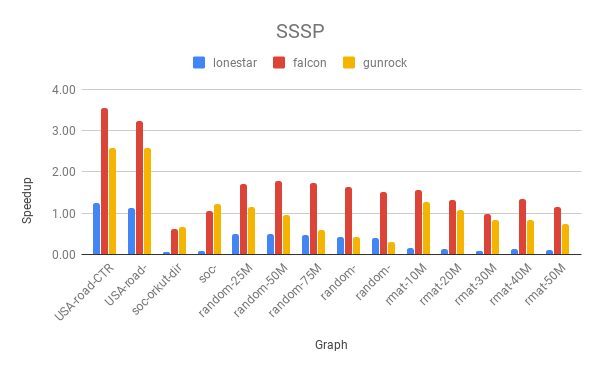
\includegraphics[width=0.99\linewidth]{SSSP.png}
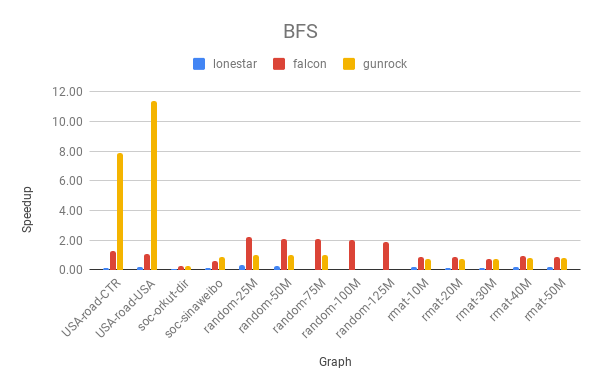
\includegraphics[width=0.99\linewidth]{BFS.png}
\caption{Falcon versus other frameworks for SSSP and BFS. Baseline is Totem at 1.0.}
\label{expt:frameworks}
\end{figure}
}

\subsection{Baselines and Comparison with Other Frameworks}\label{expt:comparison}
The baseline execution times of Falcon on GPU are listed in Table~\ref{expt:baselines}.
We observe that the execution times on road networks are particularly high for propagation based algorithms such as BFS, SSSP and CC.
This occurs because unlike other graphs, road networks have large diameters, leading to many iterations of the algorithm.


\begin{figure*}
  \begin{subfigure}{0.6\textwidth}
   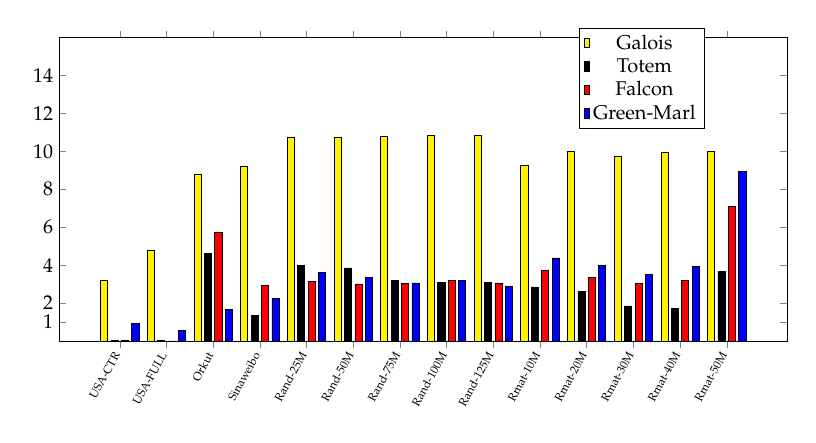
\begin{tikzpicture}[scale=0.6]
    \begin{axis}[
         ybar,% axis on top,
        ymin=0, ymax=16,
        height=8.0cm,
        width=17cm,
ytick={ 1,2,4,6,8,10,12,14},
%ymode=log,
 %       log basis y={2},
x tick label style={
rotate=60,anchor=east,font=\scriptsize},
        symbolic x coords={
           USA-CTR, USA-FULL, Orkut,Sinaweibo, Rand-25M,Rand-50M,Rand-75M,Rand-100M,Rand-125M, Rmat-10M,Rmat-20M,Rmat-30M,Rmat-40M,Rmat-50M
            },
       xtick=data,
        bar width=0.15cm,
%        major grid style={draw=black},
 %       enlarge y limits={value=.05,upper},
        % y tick style={grid=none},
         xticklabel style={rotate=1},
        %tickwidth=1pt,
       % enlarge x limits=true,
       legend style={
            at={(0.8,0.7)},
            anchor=south,
            legend columns=1,
           /tikz/every even column/.append style={font=\large}
        },
        legend entries={Lonestar-GPU,Falcon,Gunrock},
        legend image code/.code={%
      \draw[#1] (0cm,-0.1cm) rectangle (0.1cm,0.1cm);
   },  
        %ylabel={Speedup},
    %      nodes near coords,
  %nodes near coords align={vertical},
 every node near coord/.append style={color=black, rotate=90, anchor=south, font=\large},
             every axis/.append style={font=\large},
    ]
    \addplot [ fill=yellow] coordinates {
      (USA-CTR,3.18)
      (USA-FULL,4.76) 
      (Orkut, 8.77)
      (Sinaweibo,9.22)
      (Rand-25M,10.73)
      (Rand-50M,10.72) 
      (Rand-75M,10.81) 
      (Rand-100M,10.86) 
      (Rand-125M,10.86) 
      (Rmat-10M,9.28)
      (Rmat-20M,10.01) 
      (Rmat-30M,9.72) 
      (Rmat-40M,9.95) 
      (Rmat-50M,10.01) 
            };
    \addplot [ fill=black] coordinates {
      (USA-CTR,0.04)
      (USA-FULL,0.03) 
      (Orkut, 4.60)
      (Sinaweibo,1.33)
      (Rand-25M,3.97)
      (Rand-50M,3.85) 
      (Rand-75M,3.19) 
      (Rand-100M,3.08) 
      (Rand-125M,3.08) 
      (Rmat-10M,2.85)
      (Rmat-20M,2.62) 
      (Rmat-30M,1.85) 
      (Rmat-40M,1.7) 
      (Rmat-50M,3.65) 
            };
    \addplot [ fill=red] coordinates {
      (USA-CTR,0.01)
      (USA-FULL,0.00001) 
      (Orkut, 5.73)
      (Sinaweibo,2.94)
      (Rand-25M,3.16)
      (Rand-50M,3.01) 
      (Rand-75M,3.04) 
      (Rand-100M,3.2) 
      (Rand-125M,3.06) 
      (Rmat-10M,3.7)
      (Rmat-20M,3.36) 
      (Rmat-30M,3.02) 
      (Rmat-40M,3.21) 
      (Rmat-50M,7.1) 
            };
    \addplot [ fill=blue] coordinates {
      (USA-CTR,0.94)
      (USA-FULL,0.56) 
      (Orkut, 1.67)
      (Sinaweibo,2.25)
      (Rand-25M,3.61)
      (Rand-50M,3.34) 
      (Rand-75M,3.06) 
      (Rand-100M,3.2) 
      (Rand-125M,2.86) 
      (Rmat-10M,4.38)
      (Rmat-20M,3.99) 
      (Rmat-30M,3.49) 
      (Rmat-40M,3.95) 
      (Rmat-50M,8.93) 
            };
 \legend{\large{Galois},\large{Totem}, \large{Falcon},\large{Green-Marl}}
 \end{axis}
   \end{tikzpicture}
\caption{CPU: Speedup over Galois single thread}
\label{expt:ssspcpucompare}
\end{subfigure}%
  \begin{subfigure}{0.4\textwidth}
   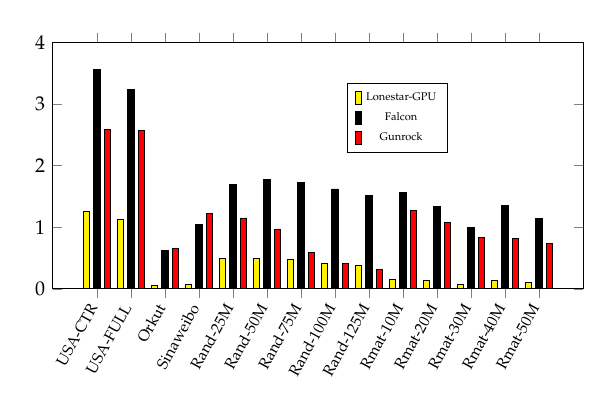
\begin{tikzpicture}[scale=0.8]
    \begin{axis}[
         ybar,% axis on top,
        ymin=0, ymax=4,
        height=5.5cm,
        width=10cm,
%ytick={0.5, 1,2,4,12,16},
x tick label style={
rotate=60,anchor=east,font=\scriptsize},
        symbolic x coords={
           USA-CTR, USA-FULL, Orkut,Sinaweibo, Rand-25M,Rand-50M,Rand-75M,Rand-100M,Rand-125M, Rmat-10M,Rmat-20M,Rmat-30M,Rmat-40M,Rmat-50M
            },
       xtick=data,
        bar width=0.1cm,
%        major grid style={draw=black},
 %       enlarge y limits={value=.05,upper},
        % y tick style={grid=none},
         xticklabel style={rotate=1},
        %tickwidth=1pt,
       % enlarge x limits=true,
       legend style={
            at={(0.65,0.55)},
            anchor=south,
            legend columns=1,
           /tikz/every even column/.append style={font=\tiny}
        },
        legend entries={Lonestar-GPU,Falcon,Gunrock},
        legend image code/.code={%
      \draw[#1] (0cm,-0.1cm) rectangle (0.1cm,0.1cm);
   },  
        %ylabel={Speedup},
    %      nodes near coords,
  %nodes near coords align={vertical},
 every node near coord/.append style={color=black, rotate=90, anchor=south, font=\tiny},
             every axis/.append style={font=\small},
    ]
    \addplot [ fill=yellow] coordinates {
      (USA-CTR,1.25)
      (USA-FULL,1.13) 
      (Orkut, 0.05)
      (Sinaweibo,0.07)
      (Rand-25M,0.49)
      (Rand-50M,0.49) 
      (Rand-75M,0.47) 
      (Rand-100M,0.42) 
      (Rand-125M,0.38) 
      (Rmat-10M,0.16)
      (Rmat-20M,0.13) 
      (Rmat-30M,0.08) 
      (Rmat-40M,0.13) 
      (Rmat-50M,0.10) 
            };
    \addplot [ fill=black] coordinates {
      (USA-CTR,3.56)
      (USA-FULL,3.23) 
      (Orkut, 0.62)
      (Sinaweibo,1.04)
      (Rand-25M,1.7)
      (Rand-50M,1.77) 
      (Rand-75M,1.72) 
      (Rand-100M,1.62) 
      (Rand-125M,1.51) 
      (Rmat-10M,1.57)
      (Rmat-20M,1.33) 
      (Rmat-30M,0.99) 
      (Rmat-40M,1.35) 
      (Rmat-50M,1.14) 
            };
    \addplot [ fill=red] coordinates {
      (USA-CTR,2.58)
      (USA-FULL,2.57) 
      (Orkut, 0.66)
      (Sinaweibo,1.22)
      (Rand-25M,1.15)
      (Rand-50M,0.96) 
      (Rand-75M,0.59) 
      (Rand-100M,0.41) 
      (Rand-125M,0.31) 
      (Rmat-10M,1.27)
      (Rmat-20M,1.08) 
      (Rmat-30M,0.83) 
      (Rmat-40M,0.82) 
      (Rmat-50M,0.73) 
            };
 \legend{Lonestar-GPU,Falcon, Gunrock}
 \end{axis}
   \end{tikzpicture}
\caption{GPU: Speedup over Totem}
\label{expt:ssspgpucompare}
\end{subfigure}%
\caption{SSSP comparison}
\label{expt:ssspcpugpu}
\end{figure*}


\begin{figure*}
\centering
  \begin{subfigure}{0.6\textwidth}
\centering
   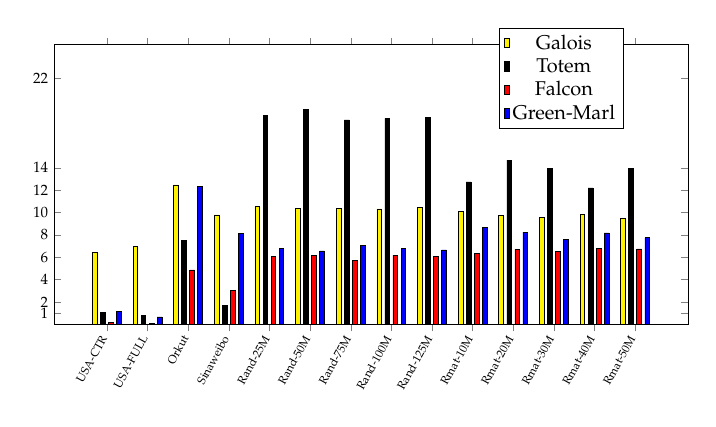
\begin{tikzpicture}[scale=0.6]
    \begin{axis}[
         ybar,% axis on top,
        ymin=0, ymax=25,
        height=7.5cm,
        width=15cm,
ytick={ 1,2,4,6,8,10,12,14,22},
%ymode=log,
 %       log basis y={2},
x tick label style={
rotate=60,anchor=east,font=\scriptsize},
        symbolic x coords={
           USA-CTR, USA-FULL, Orkut,Sinaweibo, Rand-25M,Rand-50M,Rand-75M,Rand-100M,Rand-125M, Rmat-10M,Rmat-20M,Rmat-30M,Rmat-40M,Rmat-50M
            },
       xtick=data,
        bar width=0.1cm,
%        major grid style={draw=black},
 %       enlarge y limits={value=.05,upper},
        % y tick style={grid=none},
         xticklabel style={rotate=1},
        %tickwidth=1pt,
       % enlarge x limits=true,
       legend style={
            at={(0.8,0.7)},
            anchor=south,
            legend columns=1,
           /tikz/every even column/.append style={font=\tiny}
        },
        legend entries={Lonestar-GPU,Falcon,Gunrock},
        legend image code/.code={%
      \draw[#1] (0cm,-0.1cm) rectangle (0.1cm,0.1cm);
   },  
      %  ylabel={Speedup},
    %      nodes near coords,
  %nodes near coords align={vertical},
 every node near coord/.append style={color=black, rotate=90, anchor=south, font=\tiny},
             every axis/.append style={font=\small},
    ]
    \addplot [ fill=yellow] coordinates {
      (USA-CTR,6.43)
      (USA-FULL,6.97) 
      (Orkut, 12.46)
      (Sinaweibo,9.78)
      (Rand-25M,10.51)
      (Rand-50M,10.35) 
      (Rand-75M,10.35) 
      (Rand-100M,10.32) 
      (Rand-125M,10.45) 
      (Rmat-10M,10.12)
      (Rmat-20M,9.75) 
      (Rmat-30M,9.54) 
      (Rmat-40M,9.81) 
      (Rmat-50M,9.49) 
            };
    \addplot [ fill=black] coordinates {
      (USA-CTR,1.09)
      (USA-FULL,0.82) 
      (Orkut, 7.54)
      (Sinaweibo,1.69)
      (Rand-25M,18.65)
      (Rand-50M,19.25) 
      (Rand-75M,18.28) 
      (Rand-100M,18.41) 
      (Rand-125M,18.5) 
      (Rmat-10M,12.73)
      (Rmat-20M,14.68) 
      (Rmat-30M,13.96) 
      (Rmat-40M,12.2) 
      (Rmat-50M,13.95) 
            };
    \addplot [ fill=red] coordinates {
      (USA-CTR,0.17)
      (USA-FULL,0.12) 
      (Orkut, 4.86)
      (Sinaweibo,3.01)
      (Rand-25M,6.04)
      (Rand-50M,6.16) 
      (Rand-75M,5.71) 
      (Rand-100M,6.2) 
      (Rand-125M,6.11) 
      (Rmat-10M,6.37)
      (Rmat-20M,6.73) 
      (Rmat-30M,6.54) 
      (Rmat-40M,6.77) 
      (Rmat-50M,6.75) 
            };
    \addplot [ fill=blue] coordinates {
      (USA-CTR,1.15)
      (USA-FULL,0.66) 
      (Orkut, 12.35)
      (Sinaweibo,8.1)
      (Rand-25M,6.81)
      (Rand-50M,6.57) 
      (Rand-75M,7.06) 
      (Rand-100M,6.79) 
      (Rand-125M,6.66) 
      (Rmat-10M,8.69)
      (Rmat-20M,8.24) 
      (Rmat-30M,7.57) 
      (Rmat-40M,8.17) 
      (Rmat-50M,7.76) 
            };
 %\legend{Galois,Totem, Falcon,Green-Marl}
 \legend{\large{Galois},\large{Totem}, \large{Falcon},\large{Green-Marl}}
 \end{axis}
   \end{tikzpicture}
\caption{CPU: Speedup Over Galois single thread}
\label{expt:bfscpucompare1}
\end{subfigure}%
  \begin{subfigure}{0.4\textwidth}
\centering
   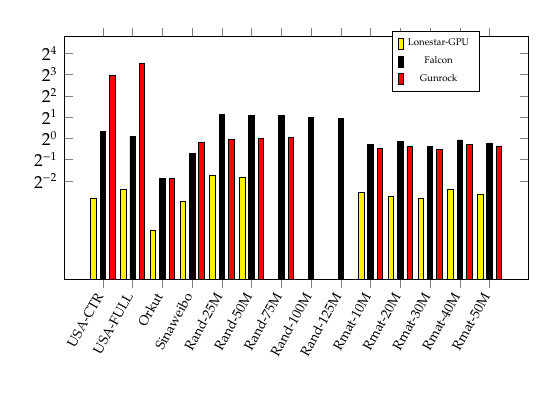
\begin{tikzpicture}[scale=0.7]
    \begin{axis}[
         ybar,% axis on top,
        ymin=0.01, ymax=28,
        height=6.0cm,
        width=10cm,
ymode=log,
log origin=infty,
        log basis y={2},
x tick label style={
rotate=60,anchor=east,font=\scriptsize},
        symbolic x coords={
           USA-CTR, USA-FULL, Orkut,Sinaweibo, Rand-25M,Rand-50M,Rand-75M,Rand-100M,Rand-125M, Rmat-10M,Rmat-20M,Rmat-30M,Rmat-40M,Rmat-50M
            },
       xtick=data,
ytick={0,0.25, 0.5, 1, 2,4,8,16},
        bar width=0.1cm,
%        major grid style={draw=black},
 %       enlarge y limits={value=.05,upper},
        % y tick style={grid=none},
         xticklabel style={rotate=1},
        %tickwidth=1pt,
       % enlarge x limits=true,
       legend style={
            at={(0.8,0.77)},
            anchor=south,
            legend columns=1,
           /tikz/every even column/.append style={font=\tiny}
        },
        legend entries={Lonestar-GPU,Falcon,Gunrock},
        legend image code/.code={%
      \draw[#1] (0cm,-0.1cm) rectangle (0.1cm,0.1cm);
   },  
        %ylabel={Speedup},
    %      nodes near coords,
  %nodes near coords align={vertical},
 every node near coord/.append style={color=black, rotate=90, anchor=south, font=\tiny},
             every axis/.append style={font=\small},
    ]
    \addplot [ fill=yellow] coordinates {
      (USA-CTR,0.14)
      (USA-FULL,0.19) 
      (Orkut, 0.05)
      (Sinaweibo,0.13)
      (Rand-25M,0.3)
      (Rand-50M,0.28) 
      (Rand-75M,0.001) 
      (Rand-100M,0.001) 
      (Rand-125M,0.001) 
      (Rmat-10M,0.17)
      (Rmat-20M,0.15) 
      (Rmat-30M,0.14) 
      (Rmat-40M,0.19) 
      (Rmat-50M,0.16) 
            };
    \addplot [ fill=black] coordinates {
      (USA-CTR,1.26)
      (USA-FULL,1.059) 
      (Orkut, 0.27)
      (Sinaweibo,0.62)
      (Rand-25M,2.2)
      (Rand-50M,2.11) 
      (Rand-75M,2.09) 
      (Rand-100M,1.98) 
      (Rand-125M,1.89) 
      (Rmat-10M,0.83)
      (Rmat-20M,0.9) 
      (Rmat-30M,0.76) 
      (Rmat-40M,0.95) 
      (Rmat-50M,0.86) 
            };
    \addplot [ fill=red] coordinates {
      (USA-CTR,7.89)
      (USA-FULL,11.39) 
      (Orkut, 0.27)
      (Sinaweibo,0.88)
      (Rand-25M,0.98)
      (Rand-50M,1.01) 
      (Rand-75M,1.02) 
      (Rand-100M,0.001) 
      (Rand-125M,0.001) 
      (Rmat-10M,0.71)
      (Rmat-20M,0.76) 
      (Rmat-30M,0.70) 
      (Rmat-40M,0.81) 
      (Rmat-50M,0.78) 
            };
 \legend{Lonestar-GPU,Falcon, Gunrock}
 \end{axis}
   \end{tikzpicture}
\label{expt:bfsgpucompare-log}
\caption{GPU: Speedup over Totem}
\end{subfigure}
\caption{BFS comparison}
\label{expt:bfscpugpu}
\end{figure*}


\begin{figure*}
  \begin{subfigure}{0.6\textwidth}
   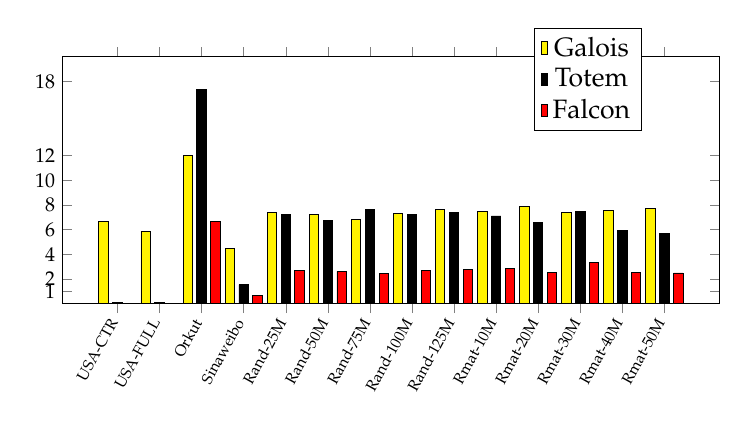
\begin{tikzpicture}[scale=0.8]
    \begin{axis}[
         ybar,% axis on top,
        ymin=0, ymax=20,
        height=5.5cm,
        width=12cm,
ytick={ 1,2,4,6,8,10,12,18},
%ymode=log,
 %       log basis y={2},
x tick label style={
rotate=60,anchor=east,font=\scriptsize},
        symbolic x coords={
           USA-CTR, USA-FULL, Orkut,Sinaweibo, Rand-25M,Rand-50M,Rand-75M,Rand-100M,Rand-125M, Rmat-10M,Rmat-20M,Rmat-30M,Rmat-40M,Rmat-50M
            },
       xtick=data,
        bar width=0.15cm,
%        major grid style={draw=black},
 %       enlarge y limits={value=.05,upper},
        % y tick style={grid=none},
         xticklabel style={rotate=1},
        %tickwidth=1pt,
       % enlarge x limits=true,
       legend style={
            at={(0.8,0.7)},
            anchor=south,
            legend columns=1,
           /tikz/every even column/.append style={font=\tiny}
        },
        legend entries={Lonestar-GPU,Falcon,Gunrock},
        legend image code/.code={%
      \draw[#1] (0cm,-0.1cm) rectangle (0.1cm,0.1cm);
   },  
        %ylabel={Speedup},
    %      nodes near coords,
  %nodes near coords align={vertical},
 every node near coord/.append style={color=black, rotate=90, anchor=south, font=\tiny},
             every axis/.append style={font=\small},
    ]
    \addplot [ fill=yellow] coordinates {
      (USA-CTR,6.67)
      (USA-FULL,5.86) 
      (Orkut, 12.01)
      (Sinaweibo,4.47)
      (Rand-25M,7.4)
      (Rand-50M,7.23) 
      (Rand-75M,6.82) 
      (Rand-100M,7.34) 
      (Rand-125M,7.62) 
      (Rmat-10M,7.5)
      (Rmat-20M,7.86) 
      (Rmat-30M,7.36) 
      (Rmat-40M,7.55) 
      (Rmat-50M,7.71) 
            };
    \addplot [ fill=black] coordinates {
      (USA-CTR,0.13)
      (USA-FULL,0.08) 
      (Orkut, 17.33)
      (Sinaweibo,1.55)
      (Rand-25M,7.25)
      (Rand-50M,6.71) 
      (Rand-75M,7.63) 
      (Rand-100M,7.26) 
      (Rand-125M,7.4) 
      (Rmat-10M,7.11)
      (Rmat-20M,6.59) 
      (Rmat-30M,7.49) 
      (Rmat-40M,5.96) 
      (Rmat-50M,5.69) 
            };
    \addplot [ fill=red] coordinates {
      (USA-CTR,0.02)
      (USA-FULL,0.02) 
      (Orkut, 6.68)
      (Sinaweibo,0.66)
      (Rand-25M,2.7)
      (Rand-50M,2.62) 
      (Rand-75M,2.44) 
      (Rand-100M,2.66) 
      (Rand-125M,2.78) 
      (Rmat-10M,2.87)
      (Rmat-20M,2.57) 
      (Rmat-30M,3.31) 
      (Rmat-40M,2.51) 
      (Rmat-50M,2.49) 
            };
 %\legend{Galois,Totem, Falcon}
 \legend{\large{Galois},\large{Totem}, \large{Falcon},\large{Green-Marl}}
 \end{axis}
   \end{tikzpicture}
\caption{CPU: Speedup over Galois single thread}
\label{expt:cccpucompare}
\end{subfigure}%
  \begin{subfigure}{0.4\textwidth}
   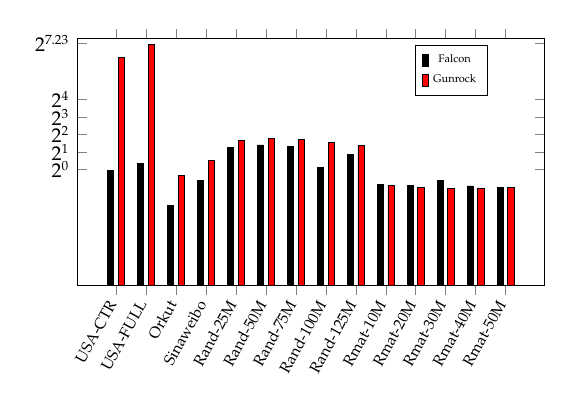
\begin{tikzpicture}[scale=0.8]
    \begin{axis}[
         ybar,% axis on top,
        ymin=0.01, ymax=180,
        height=5.5cm,
        width=9cm,
ymode=log,
log origin=infty,
        log basis y={2},
x tick label style={
rotate=60,anchor=east,font=\scriptsize},
        symbolic x coords={
           USA-CTR, USA-FULL, Orkut,Sinaweibo, Rand-25M,Rand-50M,Rand-75M,Rand-100M,Rand-125M, Rmat-10M,Rmat-20M,Rmat-30M,Rmat-40M,Rmat-50M
            },
       xtick=data,
ytick={0,1,2,4,8,16,150},
        bar width=0.1cm,
%        major grid style={draw=black},
 %       enlarge y limits={value=.05,upper},
        % y tick style={grid=none},
         xticklabel style={rotate=1},
        %tickwidth=1pt,
       % enlarge x limits=true,
       legend style={
            at={(0.8,0.77)},
            anchor=south,
            legend columns=1,
           /tikz/every even column/.append style={font=\tiny}
        },
        legend entries={Lonestar-GPU,Falcon,Gunrock},
        legend image code/.code={%
      \draw[#1] (0cm,-0.1cm) rectangle (0.1cm,0.1cm);
   },  
       % ylabel={Speedup},
    %      nodes near coords,
  %nodes near coords align={vertical},
 every node near coord/.append style={color=black, rotate=90, anchor=south, font=\tiny},
             every axis/.append style={font=\small},
    ]
    \addplot [ fill=black] coordinates {
      (USA-CTR,0.95)
      (USA-FULL,1.26) 
      (Orkut, 0.24)
      (Sinaweibo,0.65)
      (Rand-25M,2.40)
      (Rand-50M,2.65) 
      (Rand-75M,2.48) 
      (Rand-100M,1.07) 
      (Rand-125M,1.82) 
      (Rmat-10M,0.55)
      (Rmat-20M,0.53) 
      (Rmat-30M,0.64) 
      (Rmat-40M,0.52) 
      (Rmat-50M,0.49) 
            };
    \addplot [ fill=red] coordinates {
      (USA-CTR,84)
      (USA-FULL,142) 
      (Orkut, 0.78)
      (Sinaweibo,1.44)
      (Rand-25M,3.21)
      (Rand-50M,3.41) 
      (Rand-75M,3.33) 
      (Rand-100M,2.96) 
      (Rand-125M,2.63) 
      (Rmat-10M,0.53)
      (Rmat-20M,0.49) 
      (Rmat-30M,0.47) 
      (Rmat-40M,0.48) 
      (Rmat-50M,0.49) 
            };
 \legend{Falcon, Gunrock}
 \end{axis}
   \end{tikzpicture}
\caption{GPU: Speedup over Totem}
\label{expt:bfsgpucompare-log2}
\end{subfigure}
\caption{CC comparison}
\label{expt:cccpugpu}
  \end{figure*}


Figure~\ref{expt:ssspcpugpu}, Figure~\ref{expt:bfscpugpu} and Figrue~\ref{expt:cccpugpu} compares the performance of our modified Falcon against other frameworks.
For SSSP in GPU, we have observed that Falcon-generated code provides consistently better speedups compared to LonestarGPU and Gunrock, except on the two social networks (soc-orkut-dir and soc-sinaweibo).
Totem performs better on the social networks as well as on RMAT graphs due to its inbuilt edge-based processing and other optimizations to improve load-balancing across GPU threads.
In CPU version of SSSP, we have observed that Galois performs better than all other frameworks. Performance of Falcon, Totem and Green-Marl are similar.
For BFS in GPU, the results are mixed across various frameworks and there is no clear winner, but there are interesting patterns based on the graph types.
Gunrock performs quite well on the road networks (USA-road-USA and USA-road-CTR), primarily due to its work-efficient worklist-based processing.
Totem outperforms again on social networks due to edge-based processing and better load-balancing.
Performance of almost all the frameworks on RMAT graphs is quite similar, with LonestarGPU performing poorly.
Our Falcon stands out on random graphs with speedups close to 2$\times$ over all other frameworks.
In CPU, Totem is a clear winner for random and RMAT graphs whereas Galois performed better in road and social networks.
For GPU version of CC, Falcon performed better in road network, social network and random graphs. For RMAT graph, all the frameworks are similar.
In CPU version, performance of Galois and Totem are similar and better than Falcon.



\subsection{Effect of Vertex-based versus Edge-based}\label{expt:vertexedge}

\REM{
\begin{figure}
\centering
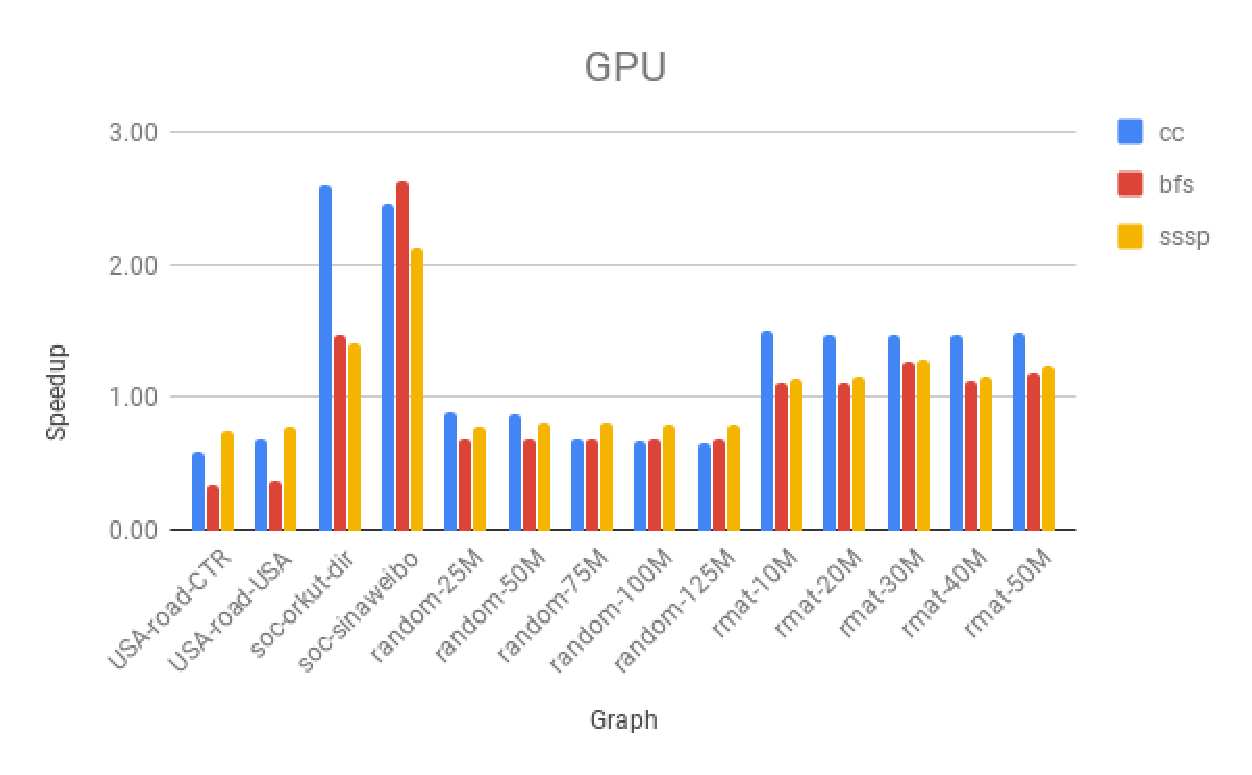
\includegraphics[width=0.99\linewidth]{GPU.pdf}
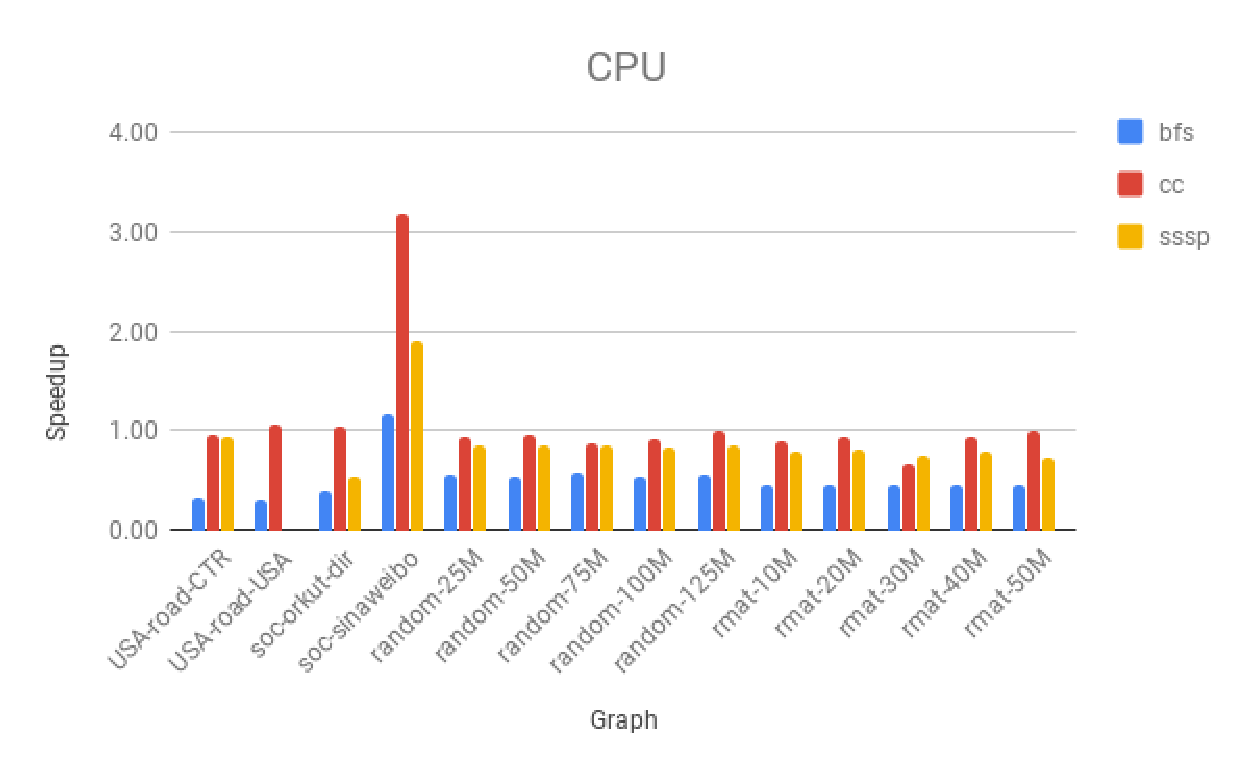
\includegraphics[width=0.99\linewidth]{CPU.pdf}
\caption{Edge-based versus vertex-based processing on GPU and CPU}
\label{speedup:gpu}
\label{speedup:cpu}
\end{figure}
}

\begin{figure*}
\centering
  \begin{subfigure}{0.45\textwidth}
  \centering
   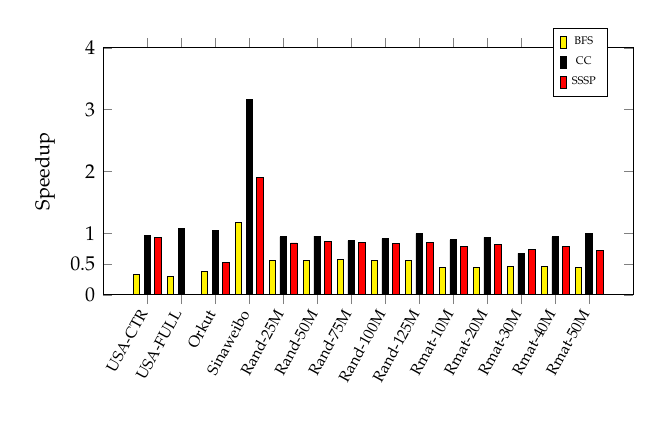
\begin{tikzpicture}[scale=0.8]
    \begin{axis}[
         ybar,% axis on top,
        ymin=0.001, ymax=4,
        height=5.5cm,
        width=10cm,
  ytick={ 0,0.5,1,2,3,4},
  x tick label style={
  rotate=60,anchor=east,font=\scriptsize},
        symbolic x coords={
           USA-CTR, USA-FULL, Orkut,Sinaweibo, Rand-25M,Rand-50M,Rand-75M,Rand-100M,Rand-125M, Rmat-10M,Rmat-20M,Rmat-30M,Rmat-40M,Rmat-50M
            },
       xtick=data,
        bar width=0.1cm,
%        major grid style={draw=black},
 %       enlarge y limits={value=.05,upper},
        % y tick style={grid=none},
         xticklabel style={rotate=1},
        %tickwidth=1pt,
       % enlarge x limits=true,
       legend style={
            at={(0.9,0.8)},
            anchor=south,
            legend columns=1,
           /tikz/every even column/.append style={font=\tiny}
        },
        legend entries={Lonestar-GPU,Falcon,Gunrock},
        legend image code/.code={%
      \draw[#1] (0cm,-0.1cm) rectangle (0.1cm,0.1cm);
   },  
        ylabel={Speedup},
    %      nodes near coords,
  %nodes near coords align={vertical},
 every node near coord/.append style={color=black, rotate=90, anchor=south, font=\normalsize},
             every axis/.append style={font=\small},
    ]
    \addplot [ fill=yellow] coordinates {
      (USA-CTR,0.33)
      (USA-FULL,0.30) 
      (Orkut, 0.38)
      (Sinaweibo,1.17)
      (Rand-25M,0.56)
      (Rand-50M,0.55) 
      (Rand-75M,0.57) 
      (Rand-100M,0.55) 
      (Rand-125M,0.56) 
      (Rmat-10M,0.45)
      (Rmat-20M,0.45) 
      (Rmat-30M,0.46) 
      (Rmat-40M,0.46) 
      (Rmat-50M,0.45) 
            };
    \addplot [ fill=black] coordinates {
      (USA-CTR,0.96)
      (USA-FULL,1.07) 
      (Orkut, 1.04)
      (Sinaweibo,3.16)
      (Rand-25M,0.94)
      (Rand-50M,0.95) 
      (Rand-75M,0.88) 
      (Rand-100M,0.91) 
      (Rand-125M,0.99) 
      (Rmat-10M,0.89)
      (Rmat-20M,0.93) 
      (Rmat-30M,0.67) 
      (Rmat-40M,0.94) 
      (Rmat-50M,0.99) 
            };
    \addplot [ fill=red] coordinates {
      (USA-CTR,0.93)
      (USA-FULL,0.0) 
      (Orkut, 0.53)
      (Sinaweibo,1.9)
      (Rand-25M,0.84)
      (Rand-50M,0.86) 
      (Rand-75M,0.85) 
      (Rand-100M,0.83) 
      (Rand-125M,0.85) 
      (Rmat-10M,0.78)
      (Rmat-20M,0.81) 
      (Rmat-30M,0.74) 
      (Rmat-40M,0.79) 
      (Rmat-50M,0.72) 
            };
 \legend{BFS,CC, SSSP}
 \end{axis}
   \end{tikzpicture}
\caption{CPU}
\label{expt:falconselfcpu}
\end{subfigure}\hfill
  \begin{subfigure}{0.45\textwidth}
      \centering
       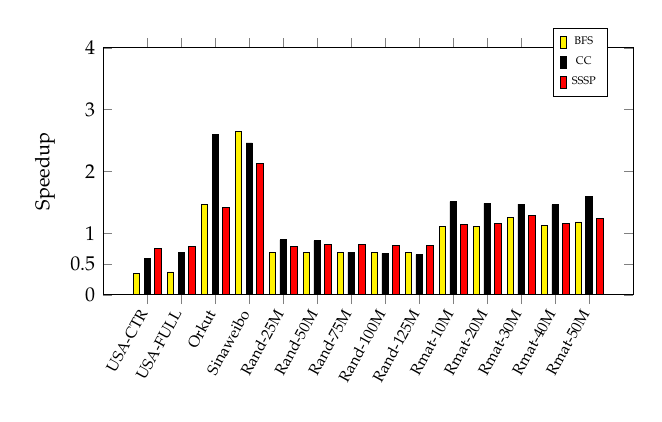
\begin{tikzpicture}[scale=0.8]
      \begin{axis}[
           ybar,% axis on top,
          ymin=0.001, ymax=4,
          height=5.5cm,
          width=10cm,
      ytick={ 0,0.5,1,2,3,4},
      x tick label style={
      rotate=60,anchor=east,font=\scriptsize},
            symbolic x coords={
               USA-CTR, USA-FULL, Orkut,Sinaweibo, Rand-25M,Rand-50M,Rand-75M,Rand-100M,Rand-125M, Rmat-10M,Rmat-20M,Rmat-30M,Rmat-40M,Rmat-50M
                },
           xtick=data,
            bar width=0.1cm,
    %        major grid style={draw=black},
     %       enlarge y limits={value=.05,upper},
            % y tick style={grid=none},
             xticklabel style={rotate=1},
            %tickwidth=1pt,
           % enlarge x limits=true,
           legend style={
                at={(0.9,0.8)},
                anchor=south,
                legend columns=1,
               /tikz/every even column/.append style={font=\tiny}
            },
            legend entries={Lonestar-GPU,Falcon,Gunrock},
            legend image code/.code={%
          \draw[#1] (0cm,-0.1cm) rectangle (0.1cm,0.1cm);
       },  
            ylabel={Speedup},
        %      nodes near coords,
      %nodes near coords align={vertical},
     every node near coord/.append style={color=black, rotate=90, anchor=south, font=\normalsize},
                 every axis/.append style={font=\small},
        ]
        \addplot [ fill=yellow] coordinates {
          (USA-CTR,0.34)
          (USA-FULL,0.37) 
          (Orkut, 1.47)
          (Sinaweibo,2.64)
          (Rand-25M,0.68)
          (Rand-50M,0.69) 
          (Rand-75M,0.68) 
          (Rand-100M,0.69) 
          (Rand-125M,0.69) 
          (Rmat-10M,1.1)
          (Rmat-20M,1.1) 
          (Rmat-30M,1.26) 
          (Rmat-40M,1.12) 
          (Rmat-50M,1.18) 
                };
        \addplot [ fill=black] coordinates {
          (USA-CTR,0.59)
          (USA-FULL,0.69) 
          (Orkut, 2.6)
          (Sinaweibo,2.46)
          (Rand-25M,0.89)
          (Rand-50M,0.88) 
          (Rand-75M,0.69) 
          (Rand-100M,0.67) 
          (Rand-125M,0.65) 
          (Rmat-10M,1.51)
          (Rmat-20M,1.48) 
          (Rmat-30M,1.47) 
          (Rmat-40M,1.46) 
          (Rmat-50M,1.60) 
                };
        \addplot [ fill=red] coordinates {
          (USA-CTR,0.75)
          (USA-FULL,0.78) 
          (Orkut, 1.41)
          (Sinaweibo,2.13)
          (Rand-25M,0.78)
          (Rand-50M,0.81) 
          (Rand-75M,0.81) 
          (Rand-100M,0.80) 
          (Rand-125M,0.80) 
          (Rmat-10M,1.14)
          (Rmat-20M,1.16) 
          (Rmat-30M,1.28) 
          (Rmat-40M,1.15) 
          (Rmat-50M,1.24) 
                };
     \legend{BFS,CC, SSSP}
     \end{axis}
       \end{tikzpicture}
    \caption{GPU}
    \label{expt:falconselfgpu}
  \end{subfigure}
\caption{Speedup of edge-based over vertex-based processing}
\label{expt:edgevertex}
\end{figure*}


Figure~\ref{expt:falconselfcpu} presents results of edge-based versus vertex-based processing of Falcon across various graphs for CC, BFS and SSSP. 
We observe that edge-based processing performs better in social-networks (soc-orkut-dir and soc-sinaweibo) and RMAT graphs. 
Both these kinds of graphs have skewed (power-law) degree-distribution resulting in large load-imbalance with vertex-based processing.
These graphs follow small-world property due to this peculiar (and natural) degree distribution.
On GPUs, this load-imbalance manifests itself as thread-divergence as the number of iterations (based on the number of neighbors) of each thread has high variance.
In other words, threads mapped to vertices having few neighbors have to wait for others mapped to high-degree vertices. 
This inhibits parallelism for SIMD style of processing.
In contrast, in edge-based processing, since threads are mapped to (a group of) edges, the load-imbalance is relatively negligible.
This results in better thread-divergence among warp-threads, leading to improved execution time.
Road networks and random graphs, on the other hand, have quite uniform degree-distribution.
Therefore, edge-based processing is not very helpful.
In fact, for uniform degree-distributions, edge-based processing may lead to inferior results (as seen in our experiments), due to increased synchronization requirement. %UK coaleased access will miss among threads in edge procesing on Graph in CSR??
Different outgoing edges of a vertex are processed sequentially by the same thread in vertex-based processing; whereas, those are processed in parallel by different threads.
Thus, edge-based processing necessitates more coordination among threads with respect to reading and updating attribute values of vertices.

Figure~\ref{expt:falconselfgpu} presents results of edge-based processing of Falcon on CPU.
We observe that, unlike on GPUs, edge-based processing is not helpful on GPUs. %UK-  GPUs->CPUs (last word in sentence
This is primarily due to CPUs not having enough resources to utilize the additional parallelism exposed by edge-based processing.
Thus, a few tens of threads perform in a similar manner in the presence of a million vertices or multi-million edges.
The only exception is soc-sinaweibo graph which witnesses over $3\times$ speedup for CC on CPU due to edge-based processing.
The improvements on this graph are also high for other algorithms as well (BFS and SSSP) compared to other graphs.
This occurs due to higher average degree in this social network (see Table~\ref{expt:chars}).%UK- orkut has more average degree ( |E| /|V|). Here |V| is low. variance in degree(1 to 33313) less   than orkut (1 to  278491).
Higher average degree adds sequentiality in vertex-based processing, while edge-based processing is not amenable to degree-distribution or average degree.
The overall effect gets pronounced for such dense graphs.

\subsection{Effect of Synchronous versus Asynchronous Processing}\label{expt:syncasync}
\begin{table}
\centering
\footnotesize
\begin{tabular}{|l|r|r|}
\hline
\textbf{Graph} & \textbf{Synchronous}  & \textbf{Asynchronous}\\
\hline
USA-road-CTR &	  86	& 91 	\\
USA-road-USA &	  134	& 106   \\
soc-orkut-dir &   425	& 285   \\
soc-sinaweibo &   8310	& 4508  \\
random-25M &   	  458	& 347   \\
random-50M &   	  945	& 741   \\
rmat-10M &   	  329	& 320   \\
rmat-20M &   	  771	& 665   \\
\hline
\textbf{Average}	&	1433	& 882	\\
\hline
\end{tabular}
\caption{Execution times (in ms) for Synchronous versus Asynchronous processing in CPU}
\label{tab:async-cpu}
\end{table}

Table~\ref{tab:async-cpu} presents the effect of asynchronous processing for various graphs on CPU.
We used a combination of BFS and SSSP to perform independent processing on the same graph.
We observe that asynchronous version improves execution time by 38\%. 
This occurs because threads do not have to wait for other threads.
This is primarily true on CPUs as threads are monolithically working on different parts of the graph and seldom require synchronization.
Such a processing is likely to benefit performance on GPUs as well, but due to limited GPU resources, the asynchronous kernels could not be executed together.
Therefore, our observed performance was the same for synchronous and asynchronous processing on GPUs (hence not shown again).

\subsection{Effect of Code Generation for Multiple Targets}\label{expt:cpugpu}

\begin{figure}
\begin{minipage}{0.45\textwidth}
\begin{table}[H]
\centering
\footnotesize
\begin{tabular}{|l|r|r|r|}
\hline
\textbf{Graphs} & \textbf{CPU-16} & \textbf{GPU} & \textbf{multi-GPU}\\\hline
random-25M + & 3866 & 1234 & 826 \\
random-50M		&	&	& \\\hline
rmat-10M + & 3024 & 1176 & 792 \\
rmat-20M	&	&	& \\
\hline
\end{tabular}
\caption{Execution time (in ms) of CC for two different graphs for various targets}
\label{tab:multigpu}
\end{table}
\end{minipage}\hfill
\begin{minipage}{0.45\textwidth}
\begin{table}[H]
\centering
\footnotesize
\begin{tabular}{|l|r|r|r|}
\hline
\textbf{Graphs} & \textbf{CPU-16} & \textbf{GPU} & \textbf{multi-GPU}\\\hline
USA-road-CTR + & 25363 & 12569 & 9138 \\
USA-road-USA	&	&	& \\\hline
soc-sinaweibo + & 4845 & 1503 & 1259 \\
soc-orkut-dir	&	&	& \\
\hline
\end{tabular}
\caption{Execution time (in ms) of BFS for two different graphs for various targets}
\label{tab:multigpumst}
\end{table}
\end{minipage}
\end{figure}

As discussed in Section~\ref{sec:cpugpu}, our approach can seamlessly generate code for CPU or GPU or multi-GPU.
The multi-GPU code works with different graphs for the same algorithm, or with the same graph for different algorithms.
Table~\ref{tab:multigpu} presents results for the former with CC as the algorithm generating code for CPU with 16 threads, single GPU and two GPUs, while Table~\ref{tab:multigpumst} presents those for BFS.
We observe that multi-GPU version took much less time as compared to other backends. 
In both CPU and single-GPU versions, the graphs are processed one after another.
On the other hand, in multi-GPU version, both the graphs are processed simultaneously in different GPUs; so the overall execution time is the larger of the two. 

\subsection{Effect of Data-Transfer Optimization}\label{expt:optimizations}
To illustrate the effect of the memcpy-optimization, we devised a simple Falcon program which computes BFS on GPU and then queries distances of various vertices from the CPU to compute the maximum distance.
We observe that the program with optimization takes less than a second to find the maximum distance.
On the other hand, without optimization the same program takes more than five minutes. 
This happens because without optimization, the existing Falcon engine generates code to copy distance of each vertex one by one as required in each iteration (total $N$ small \texttt{cudaMemcpy}s).
In contrast, the optimized code copies all the distances at once and then uses it for finding maximum distance (one large \texttt{cudaMemcpy}).
This leads to considerably reduced communication overhead, leading to improved execution.



%\subsection{Effect of Graph Type}\label{expt:graphtype}


\REM{
\begin{figure}
   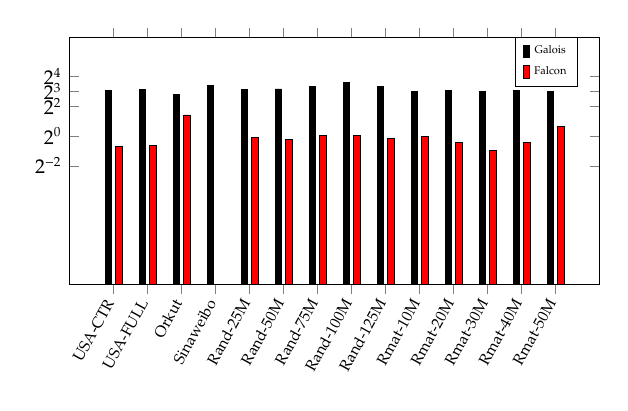
\begin{tikzpicture}[scale=0.8]
    \begin{axis}[
         ybar,% axis on top,
        ymin=0.001, ymax=100,
        height=5.5cm,
        width=10cm,
ytick={ 0.25,1,4,8,16},
ymode=log,
        log basis y={2},
log origin=infty,
x tick label style={
rotate=60,anchor=east,font=\scriptsize},
        symbolic x coords={
          % USA-CTR, USA-FULL, Orkut,Sinaweibo, Rand-25M,Rand-50M,Rand-75M,Rand-100M,Rand-125M, Rmat-10M,Rmat-20M,Rmat-30M,Rmat-40M,Rmat-50M
           USA-CTR, USA-FULL, Orkut,Sinaweibo, Rand-25M,Rand-50M,Rand-75M,Rand-100M,Rand-125M, Rmat-10M,Rmat-20M,Rmat-30M,Rmat-40M,Rmat-50M
            },
       xtick=data,
        bar width=0.1cm,
%        major grid style={draw=black},
 %       enlarge y limits={value=.05,upper},
        % y tick style={grid=none},
         xticklabel style={rotate=1},
        %tickwidth=1pt,
       % enlarge x limits=true,
       legend style={
            at={(0.9,0.8)},
            anchor=south,
            legend columns=1,
           /tikz/every even column/.append style={font=\tiny}
        },
        legend entries={Lonestar-GPU,Falcon,Gunrock},
        legend image code/.code={%
      \draw[#1] (0cm,-0.1cm) rectangle (0.1cm,0.1cm);
   },  
        %ylabel={Speedup},
    %      nodes near coords,
  %nodes near coords align={vertical},
 every node near coord/.append style={color=black, rotate=90, anchor=south, font=\normalsize},
             every axis/.append style={font=\small},
    ]
    \addplot [ fill=black] coordinates {
      (USA-CTR,8.44)
      (USA-FULL,8.88) 
      (Orkut, 7.09)
      (Sinaweibo,10.67)
      (Rand-25M,8.93)
      (Rand-50M,9) 
      (Rand-75M,10.24) 
      (Rand-100M,12.03) 
      (Rand-125M,10.11) 
      (Rmat-10M,7.94)
      (Rmat-20M,8.29) 
      (Rmat-30M,8.04) 
      (Rmat-40M,8.47) 
      (Rmat-50M,8.12) 
            };
    \addplot [ fill=red] coordinates {
      (USA-CTR,0.61)
      (USA-FULL,0.65) 
      (Orkut, 2.68)
      (Sinaweibo,0.001)
      (Rand-25M,0.92)
      (Rand-50M,0.86) 
      (Rand-75M,1.04) 
      (Rand-100M,1.03) 
      (Rand-125M,0.9) 
      (Rmat-10M,0.98)
      (Rmat-20M,0.75) 
      (Rmat-30M,0.52) 
      (Rmat-40M,0.74) 
      (Rmat-50M,1.60) 
            };
 \legend{Galois, Falcon}
 \end{axis}
   \end{tikzpicture}
\caption{MST speedup over Galois Single thread}
\label{expt:mstcpucompare}
\end{figure}
}



\REM{
  \begin{figure}
   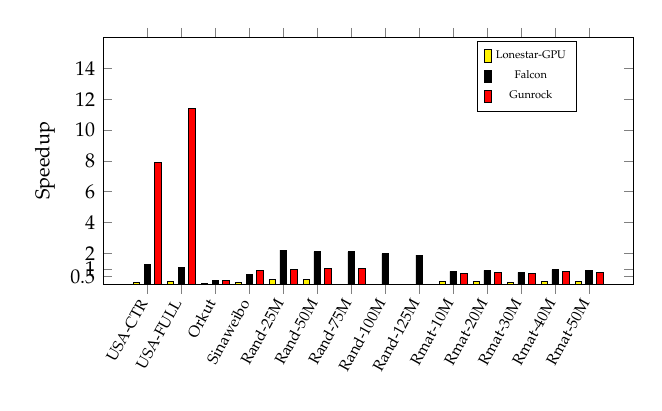
\begin{tikzpicture}[scale=0.8]
    \begin{axis}[
         ybar,% axis on top,
        ymin=0, ymax=16,
        height=5.5cm,
        width=10cm,
ytick={0.5, 1,2,4,6,8,10,12,14},
%ymode=log,
 %       log basis y={2},
x tick label style={
rotate=60,anchor=east,font=\scriptsize},
        symbolic x coords={
           USA-CTR, USA-FULL, Orkut,Sinaweibo, Rand-25M,Rand-50M,Rand-75M,Rand-100M,Rand-125M, Rmat-10M,Rmat-20M,Rmat-30M,Rmat-40M,Rmat-50M
  },
       xtick=data,
        bar width=0.1cm,
%        major grid style={draw=black},
 %       enlarge y limits={value=.05,upper},
        % y tick style={grid=none},
         xticklabel style={rotate=1},
        %tickwidth=1pt,
       % enlarge x limits=true,
       legend style={
            at={(0.8,0.7)},
            anchor=south,
            legend columns=1,
           /tikz/every even column/.append style={font=\tiny}
        },
        legend entries={Lonestar-GPU,Falcon,Gunrock},
        legend image code/.code={%
      \draw[#1] (0cm,-0.1cm) rectangle (0.1cm,0.1cm);
   },
        ylabel={Speedup},
    %      nodes near coords,
  %nodes near coords align={vertical},
 every node near coord/.append style={color=black, rotate=90, anchor=south, font=\tiny},
            every axis/.append style={font=\small},
    ]
    % \addplot [ pattern=crosshatch] coordinates {
    \addplot [ fill=yellow ] coordinates {
      (USA-CTR,0.14)
      (USA-FULL,0.19)
      (Orkut, 0.05)
      (Sinaweibo,0.13)
      (Rand-25M,0.3)
      (Rand-50M,0.28)
      (Rand-75M,0.001)
      (Rand-100M,0.001)
      (Rand-125M,0.001)
      (Rmat-10M,0.17)
      (Rmat-20M,0.15)
      (Rmat-30M,0.14)
      (Rmat-40M,0.19)
      (Rmat-50M,0.16)
            };
    \addplot [ fill=black] coordinates {
      (USA-CTR,1.26)
      (USA-FULL,1.059)
      (Orkut, 0.27)
     (Sinaweibo,0.62)
      (Rand-25M,2.2)
      (Rand-50M,2.11)
      (Rand-75M,2.09)
      (Rand-100M,1.98)
      (Rand-125M,1.89)
      (Rmat-10M,0.83)
      (Rmat-20M,0.9) 
      (Rmat-30M,0.76) 
      (Rmat-40M,0.95) 
      (Rmat-50M,0.86) 
            };
    % \addplot [ pattern=north east lines] coordinates {
    \addplot [ fill=red ] coordinates {
      (USA-CTR,7.89)
      (USA-FULL,11.39)
      (Orkut, 0.27)
      (Sinaweibo,0.88)
      (Rand-25M,0.98)
      (Rand-50M,1.01)
      (Rand-75M,1.02) 
      (Rand-100M,0.001)
     (Rand-125M,0.001)
      (Rmat-10M,0.71)
      (Rmat-20M,0.76)
      (Rmat-30M,0.70)
      (Rmat-40M,0.81) 
      (Rmat-50M,0.78) 
            };
 \legend{Lonestar-GPU,Falcon, Gunrock}
 \end{axis}
   \end{tikzpicture}
\caption{BFS speedup over Totem}
\label{expt:bfsgpucompare}
\end{figure} 
}



\newpage
\section{Related Work}\label{sec:related}
We compare with the relevant literature, by dividing it based on the type of parallel processing: multi-core, GPUs-based, and distributed.

\subsection{Multi-core CPU}
Green-Marl~\cite{Hong:2012:GDE:2150976.2151013} is a graph DSL for 
implementing parallel graph algorithms on multi-core CPUs using \texttt{OpenMP}.
 %Green-Marl has separate  data types  {\tt DGraph} and   {\tt UGraph}  for directed and undirected graphs respectively. 
It has two data types {\tt Node} and {\tt Edge} to represent vertices and edges in the graph respectively.
\REM{
 Green-Marl has three types of worklists data types namely {\tt Set}, {\tt Order} and {\tt Sequence}. These data types may contain a set of vertices in a graph. Elements in a {\tt Set} are unique but not ordered. Elements in an {\tt Order} are unique and ordered. Elements in a  {\tt Sequence} are ordered but not unique. 
Green-Marl uses {\tt Foreach} construct for parallelism.

 An example of a {\tt Foreach} statement is given below.\\

{\tt Foreach} (v : G.Nodes) (cond) \{ ... \}\\
Here all the vertices {\it v}  in the graph {\it G}  which satisfy the condition {\it cond} execute the body of the {\tt ForEach} statement. 
There are iterators for vertices ({\tt Node}) in graph like {\tt nbrs} in Green-Marl.}
 Green-Marl does not support mutation of the graph object
(i.e., adding and removing vertices and edges to/from the graph object). So dynamic graph algorithms cannot be written in Green-Marl.
LightHouse~\cite{lighthouse} added CUDA backend to Green-Marl.
\REM{ Green-Marl supports only multi-core CPUs, and  graph algorithms targeting  \GPU devices cannot be programmed in Green-Marl.}
Galois~\cite{Pingali:2011:TPA:1993316.1993501} is a C++ framework for implementing graph algorithms on multi-core CPUs. It supports mutation of graph objects via {\it cautious} speculative execution. 
It uses a {\it worklist} based execution model, where all the {\it active elements} are pushed to a {\it worklist} and are processed in {\it ordered} or {\it unordered} fashion.
\REM{Galois has a {\tt foreach} operator to process active elements in parallel. 
The {\tt foreach} operator takes as argument an  {\it ordered} or {\it unordered} worklist.
 During the processing of {\it active elements}, new {\it active elements} are created, which will be processed in the following rounds of computation. }
Elixir~\cite{Prountzos:2012:ESS:2398857.2384644} is  a graph DSL to  develop and implement parallel graph algorithms for analyzing static (i.e., non-mutable) graphs and it targets multi-core CPUs.
\REM{ Elixir uses both declarative and imperative  constructs for determining computations over a graph. }

X-Stream~\cite{Roy:2013:XEG:2517349.2522740}  uses edge-centric processing for graph applications.
\REM{ rather than using vertex centric processing for algorithms such as SSSP and Strongly Connected Component (SCC)}. 
It supports both in-memory and out-of-core graph processing on a single shared-memory machine using scatter-gather execution model.
The Stanford Network Analysis Platform (SNAP)~\cite{Leskovec:2016:SGN:2973184.2898361} provides high-level operations for large network analysis including social networks and target
multi-core CPUs. 
Ligra~\cite{Shun:2013:LLG:2517327.2442530} is a framework for writing graph traversal algorithms
for multi-core shared memory systems. For vertex- versus edge-based processing, it uses two different routines: one for  mapping  vertices and the other for mapping  edges. However, the DSL code needs modification if one needs to alter the mapping.
Polymer~\cite{Zhang:2015:NGA:2858788.2688507} is a NUMA aware graph framework for multi-core CPUs and it is built
with a hierarchical barrier to get more parallelism and locality. 
The GraphChi~\cite{Kyrola:2012:GLG:2387880.2387884} framework processes large graphs using a
single machine, with the graph being split into  parts, called shards, and loading shards one by one into RAM and then processing each shard. 
Such a framework is useful in the absence of distributed clusters.

\subsection{\GPU devices}
 Due to {\it irregularity} present in the graph algorithms  thread divergence can happen in \GPU.
\REM{Writing an efficient \GPU program requires a deep knowledge of the \GPU architecture, so that the algorithm can be implemented with less thread divergence, fewer atomic operations, coalesced access etc.}
Past research  has shown that graph algorithms perform well on GPUs and much better than multi-core \CPU  even in the presence of   the above mentioned limitations. 
 The BFS implementation from  Merrill~\cite{Merrill:2012:SGG:2370036.2145832} is  novel and efficient. 
There have also been successful implementations of other local computation algorithms such as 
betweenness centrality~\cite{sariyuce13} and data flow analysis ~\cite{mendezlojo12}  on \GPU.
Different ways of writing SSSP programs (such as delta-stepping~\cite{meyer03}) on
\GPU along with their merits and demerits have been explored in~\cite{DAVIDSON2014} and it  concludes that worklist-based implementation will
not benefit much on \GPU compared to that on a \CPU.

The Lonestar-GPU~\cite{nasre13:MAG:2517327.2442531} framework supports mutation of graph objects and implementation of cautious morph algorithms on \GPU.
It has cautious morph implementations  of algorithms like  Delaunay Mesh Refinement, Survey Propagation and  Points-to-Analysis. 
\REM{ Lonestar-GPU does not provide any API based programming style for GPUs and it does not support execution of an algorithm  on   multiple GPUs by graph partitioning or running different algorithms at the same time.}
 Medusa~\cite{medusa2014} is a  programming framework for graph algorithms on GPUs and multi-GPU devices. 
It provides a set of  APIs and a run time system to program graph algorithms targeting GPU devices.
The programmer is required  to write only  sequential {\it C++} code with these APIs. 
\REM{Medusa provides APIs  for  processing vertices, edges or messages on GPUs.
A programmer can implement an algorithm using these APIs.}
 APIs on vertices and edges can also send messages to neighboring vertices.
The Gunrock~\cite{Wang:2016:GHG:3016078.2851145} framework provides  a data-centric abstraction for graph operations at
a higher level which makes programming  graph algorithms easy.
Gunrock has  a set of  APIs to  express a  wide range of graph processing primitives.
Gunrock also has some  GPU-specific optimizations.
\REM{It defines {\it frontiers} as a subset of edges and  vertices of the graph  which are actively involved in the computation.
Gunrock defines {\it advance}, {\it filter}, and {\it compute} primitives which operate on {\it frontiers} in different ways.}
In Gunrock, programs can be specified as a series of bulk-synchronous steps. 
\REM{Gunrock also looks at GPU specific optimizations such as kernel fusion.
Gunrock provides load balance on irregular graphs where the {\it degree} of the vertices in the {\it frontier} can vary a lot.
This variance is very high in graphs which follow power-law distribution.}
Totem~\cite{Gharaibeh:2012:YOT:2370816.2370866,Gharaibeh:2013:ECG:2535753.2535755} is a heterogeneous framework for graph processing on a single machine.  It supports using a multi-core CPU and multiple GPUs on a single machine.
\REM{When multiple devices are used for computation, the graph is partitioned and stored in the devices used for computation.}
Totem follows the Bulk Synchronous Parallel~\cite{Valiant:1990:BMP:79173.79181} model of execution.
\REM{Computation happens in a series of supersteps called {\it computation}, {\it communication} and {\it synchronization}.
 It  supports large-scale graph processing on a single machine.}
IrGL~\cite{Pai:2016:CTO:2983990.2984015} implements three optimizations named {\it iteration outlining}, {\it cooperative conversion} and
 parallel execution of nested  loops. IrGL is an intermediate code representation, on which these optimizations are applied and the CUDA code is generated from it. \REM{ {\it Iteration outlining}  moves the 
iterative loop from the {\it host} code  to the {\it device} code and this eliminates the performance bottleneck associated with multiple kernel calls in an iterative loop. 
  {\it Cooperative conversion} reduces the total number of  atomic operations  by aggregating functions over thread, warp and thread-block level.\par}
Farzad et al.~\cite{Farzad2016} propose warp segmentation to improve  GPU  utilization by
dynamically assigning appropriate number of threads to process a vertex.
GasCL (Gather-Apply-Scatter with OpenCL)~\cite{GasCL2013}  is a graph processing framework  built on top of
OpenCL which works  on several  accelerators and supports parallel work distribution and message passing.
The  MapGraph~\cite{Fu:2014:MHL:2621934.2621936}  framework  provides  high-level APIs, making it easy  to write graph programs and obtain good  speedups on GPUs.
 Halide~\cite{Ragan-Kelley:2013:HLC:2491956.2462176} is a programming model for image processing on CPUs and GPUs.
 An online profiling based method~\cite{Kaleem:2014:AHS:2628071.2628088} partitions work and distributes it across CPU and GPU.
CuSha~\cite{Khorasani:2014:CVG:2600212.2600227}  proposes two new ways of storing graphs on GPU called G-Shards and Concatenated Windows,  that have improved regular memory access patterns.
OpenMP to GPGPU~\cite{Lee:2009:OGC:1594835.1504194} is a framework for automatic code generation
for GPU from OpenMP CPU code. There is no support from the CUDA compiler to have a barrier for the all threads in a {\it kernel} blocks. Such a feature is needed in some {\it cautious} morph algorithm (e.g, DMR). 
A barrier for all the threads in a {\it kernel} can be  implemented in software, by launching the {\it kernel} with less number of threads and 
 with the help of {\it atomic} operations provided by CUDA, and  each thread processes a set of elements.
 Such an implementation can be found in~\cite{Feng5470477}. 
\subsection{Distributed Systems}
Natural graphs have very big sizes. Such large-scale graphs are sparse and follow the power-law degree distribution. Such graphs are
 processed on a computer cluster.  Programming for a computer cluster requires learning the MPI library and explicit communication code
has to be inserted in the program, with proper synchronizations to preserve sequential consistency. To achieve good performance
there should be work balance across machines in the cluster and communication overhead should be minimum. Also the graph  should be
partitioned across machines with less storage overhead.
GraphLab~\cite{Low:2012:DGF:2212351.2212354}, PowerGraph~\cite{Gonzalez:2012:PDG:2387880.2387883} and Pregel~\cite{Malewicz:2010:PSL:1807167.1807184}  are popular distributed graph analytics framework.
 Bulk Synchronous Parallel (BSP) Model  \cite{Valiant:1990:BMP:79173.79181} of execution and asynchronous executions are popular models of executions.
Giraph~\cite{Ching:2015:OTE:2824032.2824077} is an  open source framework written in {\it Java} which is  based  on the Pregel model and runs on the  Hadoop infrastructure.
 GPS (Graph Processing System)~\cite{Salihoglu:2013:GGP:2484838.2484843} is an open source
framework and follows the execution of model of Pregel. 
Green-Marl compiler was extended to CPU-clusters~\cite{Hong:2014:SSG:2581122.2544162}  and
it generates GPS based Pregel like code.
 Mizan~\cite{Khayyat:2013:MSD:2465351.2465369}  uses
dynamic monitoring of algorithm execution, irrespective of graph
input and does vertex migration at run time to balance computation and communication.
Hadoop~\cite{White:2009:HDG:1717298}  follows the MapReduce() processing
of graphs and uses the  Hadoop distributed file system (HDFS)
for storing data.
\REM{ HaLoop~\cite{Bu:2010:HEI:1920841.1920881} is a framework which follows
MapReduce() pattern with support for iterative computation
and with better caching and scheduling methods.}
 Pregel like systems can outperform MapReduce() systems in graph analytic applications.
Gluon~\cite{Dathathri:2018:GCS:3192366.3192404} uses Galois and Ligra and generates distributed-memory versions of these systems.
 Gemini~\cite{Zhu:2016:GCD:3026877.3026901} is a distributed graph processing framework and provides abstractions for push-pull model of computation on distributed systems.

\newpage
\section{Conclusion}\label{sec:conclusion}
Irregular codes have data-dependent access patterns.
Therefore, compilers need to make pessimistic assumptions leading to very conservative code.
While DSLs for irregular codes allow us the flexibility to make more informed decisions about the domain, existing DSLs lack adaptability.
Different graphs expect different kinds of processing to achieve the best performance.
While existing DSLs do allow changing the algorithm specification to be changed to suit a purpose, it would be ideal if the specification remains intact and the compiler judiciously generates the necessary efficient code.
We presented our experiences in achieving the same, for a graph DSL, Falcon.
In particular, we auto-generated codes for vertex-based and edge-based processing, for synchronous versus asynchronous processing, and for CPU versus GPU versus multi-GPU processing.
We illustrated the effectiveness of our techniques using a variety of algorithms and several real-world graphs.
We believe other DSLs would also benefit from our proposal.


\newpage
\bibliographystyle{plain}
\bibliography{ref}
\end{document}



